\documentclass[times,12pt]{article}
\usepackage{amsmath,amssymb,amsthm,mathrsfs,graphicx}
\usepackage{titlesec}
\usepackage{algorithm}
\usepackage{color}
\usepackage{float}
\usepackage{graphicx}
\usepackage{rotating}
\usepackage{url}
\usepackage{fancyhdr}

\usepackage{algorithmicx, algorithm, algpseudocode}
\floatname{algorithm}{Algorithm}

\pagenumbering{arabic}

\setlength{\parindent}{0pt}
\setlength{\parskip}{5pt plus 2pt minus 1 pt}

\topmargin  -15mm
\evensidemargin 0mm
\oddsidemargin  0mm
\textwidth  160mm
\textheight 235mm
\frenchspacing
\sloppy
\titlespacing{\section}{0pt}{\parskip}{0.01\parskip}
%%%%%%%%%%%%%%%%%%%%%%%%%%%%%%%%%%%%%%%%%%%%%%%%%%%%%%%%%%%%%%%%%%%%%%%

\begin {document}

\pagestyle{plain}

\begin{center}
{\fontsize{22}{20}\bf A Parallel Grid-based Approach for Multiscale Non-Spherical Geometry Impact Dynamics\\
}\end{center}

\vspace{\fill}
\begin{center}\fontsize{16}{20}
\textbf{Konstantinos Krestenitis$^1$}\\
\today
\end{center}
\vspace{\fill}

\begin{center}
{\fontsize{10}{12}
}\end{center}

\begin{center}
$^1$School of Engineering and Computing Sciences, University of Durham, DH1 3LE, Durham\\
konstantinos.krestenitis@durham.ac.uk\\
Mechanics Research Group\\
\end{center}
\begin{center}
Supervised by\\
Dr Tobias Weinzierl\\
Dr Tomasz Koziara (former)\\
Professor Jon Trevelyan\\
\end{center}

\clearpage

\section{Introduction}
We present a Discrete Element Method (DEM) contact detection code that simulates rigid non-spherical particles on manycore shared memory machines and distributed memory computers. DEM is used to study granular particles in fields like soil mechanics. We rely on triangulated particle meshes to model surfaces. Spherical or multi-sphere models currently are state-of-the-art - due to a lack of well-suited software and runtime demands. Non-spherical particles promise to facilitate more accurate physics than sphere-based approaches \cite{AlonsoMarroqu2013}. The focus on triangles for rigid contact mechanics facilitates memory layouts allowing vectorised computation \cite{Alvarez2007, Koziara2005, Krestenitis2015}. It is vital to yield high performance on current and upcoming processor architectures to enable engineers to simulate more realistic materials.

It is important to investigate the problem of finding the minimum distance between triangles because of the changes in the computational hardware \cite{Dongarra2011}. The central processing unit architecture today and the future upcoming hardware support Single Instruction Multiple Data (SIMD)\cite{Alvarez2007} parallelism which allow data level parallelism. These speed-ups are enabled because of new instruction sets and wide vector register. Furthermore, shared memory parallelism at the node level as well as distributed memory for supercomputers can provide significant speed-ups. It is vital to extract resources available on current and upcoming hardware, the speed-ups enable more triangles to be used to describe surfaces. Consequently, our objective is to enable engineers to use an algorithm that is capable to handle the maximum amount of triangles per time step to do better engineering and science.

In the present work we propose a hybrid method that combines the advantages of two optimised triangle-to-triangle distance computation methods. It benefits from both performance and robustness of an iterative Newton-penalty and a brute force solver. We exploit shared memory parallelism and SIMD (Single Instruction Data) to perform contact detection at the node level. On distributed memory, we use spatial domain decomposition  whilst with the Message Passing Interface (MPI), we exploit asynchronous non-blocking communication to overlap data exchange with computation.

The state-of-the-art large scale DEM work, to the best of my knowledge, relies on sphere-based or multi-sphere particles \cite{Gonnet2013, Gonnet2014}. Large scale applications of spherical particles can be found in the field of molecular dynamics. Large scale non-spherical particle based DEM simulations in literature \cite{Girolami2012, Iglberger2009, Iglberger2010, Iglberger2011} often describe particles as convex polyhedra and contact detection is resolved with GJK (Gilbert-Johnson-Keerthi) \cite{Ericson2005} variants which require interpenetration and access to all vertices of the particle to detect contact on the surface. Interpenetration introduces contact point clustering and the problem of divergence \cite{Koziara2008, koziara2011, Krestenitis2015}. In addition, convex polyhedra based contact detection methods require undeterministic memory access to all particle simplices \cite{Ericson2005} which is contradictory to the aligned memory access imposed by SIMD for data locality. Triangle-based contact detection retain locality for vectorisation as well as increases accuracy of contact point generation \cite{Krestenitis2015}. Furthermore, the method can be extended to run on shared memory manycore and distributed memory machines.

The remainder of the paper is structured as follows. In Section 2, we describe the serial DEM  algorithm. In Section 3 we review two triangle-to-triangle distance algorithms. We create a new hybrid shared memory method that benefits from fast convergence and robustness. Next, in Section 3, we propose a distributed memory algorithm for contact detection that use asynchronous communication to overlap computation over communication. Section 4, discusses the future research directions.

\section{Algorithmic Overview}
\vspace{5mm}
\begin{itemize}
\item Completed since last report: Implemented serial DEM simulation with triangle-to-triangle contact detection using spring-dashpot contact forces, explicit time step.
\item New concepts: New shared memory hybrid method for computation of triangle-to-triangle distance.
\item Open questions: Best-case design of distributed memory implementation is not clear yet, real-world experiments are missing.
\end{itemize}

In contact mechanics, fluid-stucture interaction or other fields, it is an essential task to compute the distance between geometries to determine contact. Contact detection also is the most expensive algorithmic step \cite{Koziara2010, Wachs2012}. We present a Discrete Element Method (DEM) code that simulate particles that interact with spring-based contact. Non-spherical particles promise to facilitate more accurate physics than sphere-based approaches \cite{AlonsoMarroqu2013, Girolami2012}. The contact detection routine determines contact based on the distance between the triangles of every particle against all other. If two triangles are closer than a prescribed threshold, they are considered to contact each other. The use of triangles for rigid body contact dynamics rather than arbitrary polygons simplifies geometric checks and facilitates memory layouts that allow vectorised computation \cite{Eichenberger2004, Juurlink, Krestenitis2015, Krestenitis2016}.

The serial DEM Algorithm \ref{alg1} demonstrates the execution of contact detection, an O($n^2$) operation. In line 3 and line 4 the nested for loop indicate the complexity of iterating through all triangle pairs. In line 5 TTD(i, j) invokes a Triangle-to-Triangle Distance (TTD) algorithm that determines the distance between triangle i and triangle j. Based on the boundary layer margin contact model \cite{Krestenitis2015} to avoid penetration, we check if distance between Triangle i and j is smaller than a set margin (line 6). If the parent particle of triangle i and j is not the same then this indicate a contact point between the two particles (line 7). The contact point information at line 13 and line 14 is used to derive the forces. The forces accelerate the particles that are then integrated by an explicit time stepping scheme such as explicit Euler.

\clearpage

\begin{algorithm}	

1 \textbf{\textcolor{blue}{FOR}} time = 0; time $<$ simulation time; time+=step

2~~~//contact detection
		
3~~~~~~	\textbf{\textcolor{blue}{FOR}} i = 0 to N triangles

4~~~~~~~~~\textbf{\textcolor{blue}{FOR}} j = i+1 to N triangles
				
5~~~~~~~~~~~~distance = TTD(i,j)
				
6~~~~~~~~~~~~\textbf{\textcolor{blue}{IF}} (distance $<$ margin) AND ParticleID(i) != ParticleID(j)

7~~~~~~~~~~~~~~~contact(PID(i)).add(point, normal)

8~~~~~~~~~~~\textbf{\textcolor{blue}{ENDIF}}
			
9~~~~~~~~~\textbf{\textcolor{blue}{	ENDFOR}}
			
10~~~~~~\textbf{\textcolor{blue}{ENDFOR}}

11~~~//force derivation
		
12~~~~~~\textbf{\textcolor{blue}{FOR}} z = 0 to NB particles

13~~~~~~~~~	\textbf{\textcolor{blue}{FOR}} k = 0 to contacts(z).size()

14~~~~~~~~~~~~~~~force = granular(velocity(z), position(z), contacts(z).getcontact(k))

15~~~~~~~~~	\textbf{\textcolor{blue}{ENDFOR}}

16~~~~~~\textbf{\textcolor{blue}{ENDFOR}}
	
17~~~//explicit time stepping

18 \textbf{\textcolor{blue}{ENDFOR}}

\protect\caption{\label{alg1}DEM Serial Simulation Pseudo code}
\end{algorithm}


\begin{algorithm}	
  0 \textbf{\textcolor{blue}{FUNCTION}} force = penaltyForce(normal, relativeVelocity, depth, massA, massB)
  
  1~~mass = 1.0 / ((1/massA) + (1/massB));
  
  2~~velocitymagnitude = DOT(relativeVelocity, normal);
  
  3~~magnitude = SPRING*depth + DAMPER*sqrt(SPRING*mass)*velocitymagnitude;
  
  4~~force = magnitude*normal;
  
  5 \textbf{\textcolor{blue}{ENDFUNCTION}}
\protect\caption{\label{alg2}Spring-dashpot force algorithm}
\end{algorithm}

Algorithm \ref{alg2} shows the spring-based force derivation approach \cite{Koziara2008, solberg2000, Wachs2012, Williams1999}. To define contact points without penetration, we use the boundary layer margins to extend the surface boundary. Margin size is set based on velocities and time step size. When in contact, the margin overlap is used as the interpenetration depth. The contact point is at the middlepoint of the distance and normal direction is either side of the distance. At line 0, given the contact point normal, relative linear velocities, penetration depth and the mass of the two bodies we derive the interaction force to update the position of particle triangles on every time step.

\clearpage


\section{Grid meta data structures}
\label{section:grid}

Various speedup techniques such as linked-cell lists \cite{Eckhardt2014} and Verlet lists
\cite{Fleissner, Eckhardt2014} reduce the quadratic complexity in DEM codes.
We propose to rely on a generalised tree-based linked-cell
technique that allows us to efficiently treat particles from a vast range of diameters.
Three observations support this design decision:
First, particles colliding with other particles are close to these particles.
It is sufficient to scan a certain environment around each particle for
potential collision partners.
We thus split up the domain into control volumes.
They are cubic as this simplifies the implementation compared to control volumes
of more flexible shapes.
Second, we may choose these control volumes to be larger than the biggest
particle diameter. 
For a particle held in a particular control volume (cell), it is thus sufficient
to check the $3^d-1$ neighbouring cells whether they host other particles that
might collide. 
$d$ is the spatial dimension.
Third, the previous decision is problematic if the particles are of extremely
different size. 
The cell size is determined by the largest particle diameter. 
If we use a uniform cell size, many unnecessary collision checks are performed
for small particles.
If we use an adaptive grid, it is tricky to design the grid such that only
direct neighbouring cells have to be studied.
We thus, third, observe that a cascade of grids might be useful: If we have
several grids embedded into each other, we can store each particle in the grid
suiting its diameter.
Particles of one grid then have to be checked agains particles in their
neighbouring cell as well as neighbouring cells on coarser grid resolution
levels.
There is no need to check a particle of one grid resolution with particles of a
finer grid resolution---if a particle $A$ collides with a particle $B$, particle
$B$ also collides with particle $A$ and such relations thus are already
detected.

A spacetree is a space-partitioning data structure constructed recursively.
The computational domain is embedded into a unit cube.
We cut the unit cube into three equidistant pieces along each coordinate axis. 
This yields 27 new cubes. 
They are called children of the bounding box cube which is the root.
For each of the children, we continue recursively to evaluate the split
decision. 
The decision to cut into three parts results from the fact that we rely on a
code base based upon three-partitioning \cite{Software:Peano}.
Bipartitioning, i.e.~the classic octree, works as well.


The construction scheme yields a cascade of ragged regular Cartesian grids that
are embedded into each other.
Each cell besides the root has a unique parent cell.
While we could make the cells hold particles, we propose to use a
multiscale, vertex-based scheme spanning a dual meta grid
\cite{Weinzierl:16:PIC}.
A vertex is unique through its spatial position plus its level. 
The level is the number of refinement steps required at least to create one of
its adjacent cells.
Each vertex holds a list of particles.
A particles is always stored on the finest grid level where the cells' edge
length is still bigger than its diameter.
A particle is always associated to the vertex next to its geometric centre,
i.e.~any vertex has a list of all particles close to it on the same level.
Links from the vertices to the particles are realised as pointers. 
If a particle moves, we have to update the links, but we do not move
geometric data in memory.

%{\bf Grid traversal.}
With a grid at hand, we may map the algorithmic steps from Algorithm
\ref{algorithm:dem-blueprint} onto a grid traversal.
For the traversal, we rely on a combination of a depth-first order with
space-filling curve \cite{Weinzierl:2009:Diss,Weinzierl:11:Peano}.
From a DEM point of view, the exact traversal realisation however is not that
relevant as long as the traversal is a real tree traversal, i.e.~runs through
all levels of the underlying spacetree.

\begin{figure}
  \begin{center}
    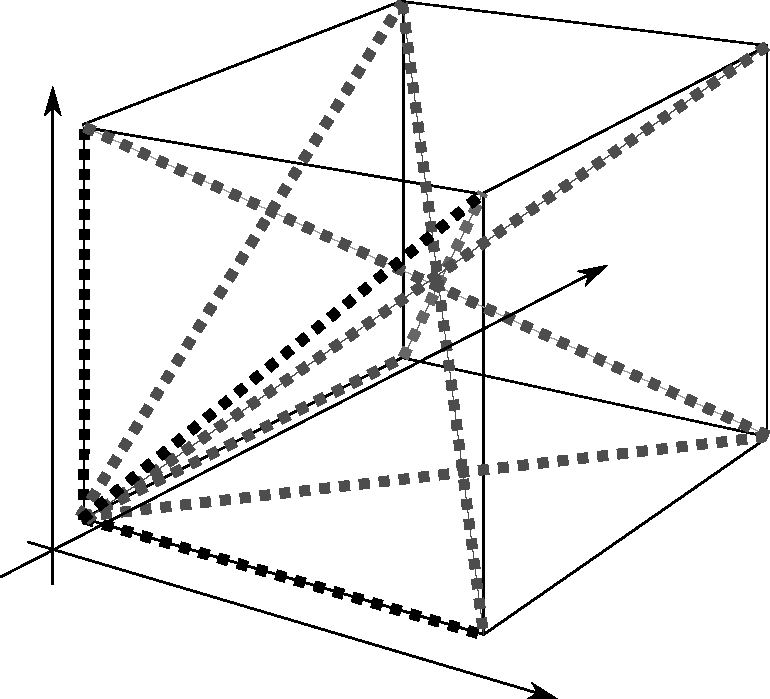
\includegraphics[width=0.25\textwidth]{sketches/collision-cube.pdf}
    \hspace{0.2cm}
    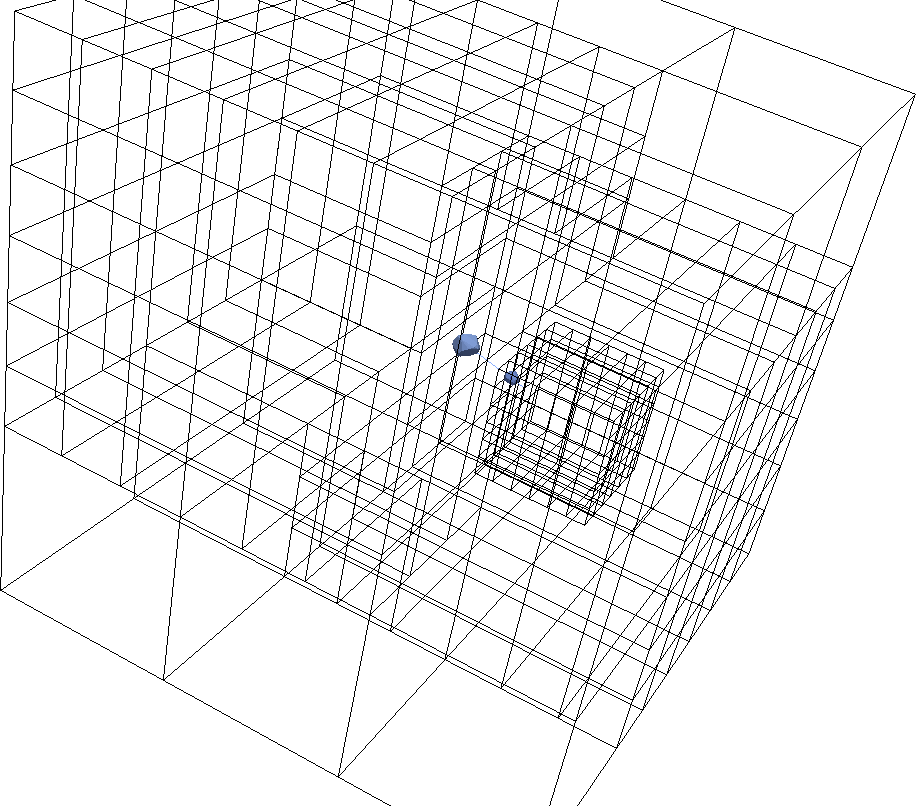
\includegraphics[width=0.3\textwidth]{experiments/two-bodies/visualisation/adaptive-grid01.png}
    \hspace{0.2cm}
    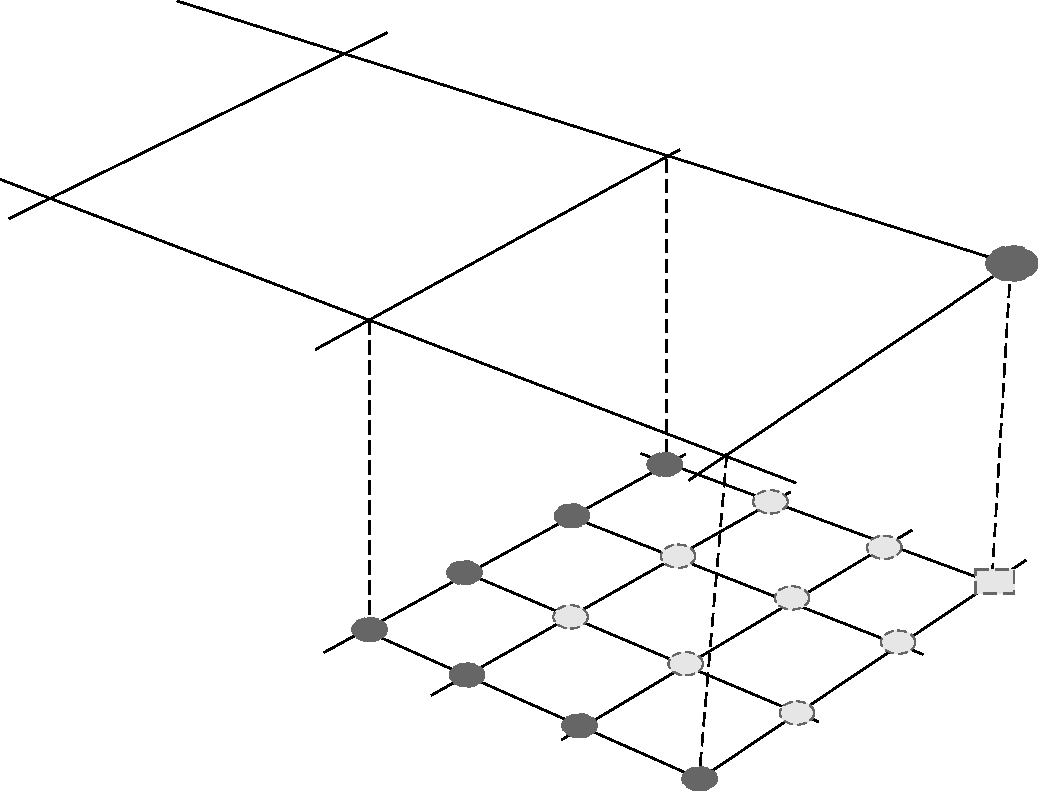
\includegraphics[width=0.3\textwidth]{sketches/multigrid.pdf}
  \end{center}
  \caption{
    Left: Whenever the grid traversal enters a cell, it checks whether particles
    assigned to one vertex do collide with particles assigned to another vertex.
    To avoid redundant collision computations, we check only some vertex pairs
    (dotted, larger lines).
    Middle: Two particles approach each other. As they are of different size,
    they might be held on different spacetree resolution levels.
    Right: In the adaptive case, particles are dropped from the coarse levels
    into the fine grid (rectangular marker) if new grid levels are added. The
    bright round vertices are children of the marked coarse grid vertex. The
    bright and the dark round markers' vertices together are the descendants of
    the marked coarse grid vertex.
  }
  \label{figure:collision-cube}
\end{figure}


We then write down the algorithm as a set of events, i.e.~we specify which
operations are performed if a vertex is read for the very first time \linebreak
(\texttt{touchVertexFirstTime}), if a cell is entered
(\texttt{enterCell}), and so forth.
Besides the actual grid hosting the particles, the grid sweeps build and
maintain two further sets of collision points (algorithm \ref{algorithm:grid-based-dem}).


\begin{algorithmic}[1]
  \Function{traverseGrid}{$\mathcal{C}$}
   \State $\mathcal{C}_{old} \gets \mathcal{C}$
   \State $\mathcal{C} \gets \emptyset$
   \While{traversal continues}
    \If{\texttt{touchVertexFirstTime}}
     \ForAll{particles $p$ associated to vertex}
      \ForAll{contact points $c \in \mathcal{C}_{old}$ associated to $p$}
       \State Update $f(p)$ through $c$
      \EndFor
      \State Update particle incl.~its triangles
     \EndFor
     \ForAll{particle pairs $(p_i,p_j)$ associated to vertex}
       \State $\mathcal{C} \gets \mathcal{C} \cup $
       \Call{findCollisions}{$p_i,p_j$}
     \EndFor
    \EndIf
    \If{\texttt{enterCell}}
     \ForAll{$2^d$ vertices adjacent to cell}
      \ForAll{particles $p$ associated to vertex}
       \If{particle should be associated to different vertex}
        \State Reassign particle
       \EndIf
      \EndFor
     \EndFor
     \ForAll{$(p_i,p_j)$ associated to different vertices (cmp.~figure)} 
      \State $\mathcal{C} \gets \mathcal{C} \cup $
       \Call{findCollisions}{$p_i,p_j$}
     \EndFor
    \EndIf
   \EndWhile
  \EndFunction

  %\Function{main}{$T$}   
  % \State $\mathcal{C} \gets \emptyset $
  % \State $t \gets 0 $
  % \For{$t < T$}
  %  \State \Call{traverseGrid}{$\mathcal{C}$}
  %  \State $t \gets t + \Delta t$
  % \EndFor
  %\EndFunction
  
 %\caption{A grid-based DEM implementation.}
 \label{algorithm:grid-based-dem}
\end{algorithmic}


Our grid-based realisation is characterised by few properties:
\begin{itemize}
  \item When we load a vertex for the very first time, we make all particles
  associated to this vertex move. 
  \item When we load a vertex, we do compare all the particles associated to
  this vertex with each other and identify collision points. The comparison of
  particles associated to different vertices is realised when we enter a cell.
  Here, we do compare the vertex pairs from Figure \ref{figure:collision-cube}---left bottom
  front vertex with right bottom front vertex, all diagonal combinations, and
  so forth---such that we avoid multiple evaluations of vertex pairs. For 
  boundary cells, some special case distinctions yielding additional checks are
  added. If a cell is traversed, we assume that all its adjacent vertices are
  available, i.e.~have been read before.
  \item Whenever we run into a cell, we run through all the adjacent vertices
  and their particles. They all already have an updated position, as any vertex
  has been loaded before and thus been subject to \texttt{touchVertexFirstTime}.
  If a particle is associated to the 'wrong' vertex as it has moved and should 
  be assigned to another vertex of the cell, we do the reassignment. A particle
  may move at most one cell of its corresponding level a time.
  \item The vertex comparisons yield a set of collision points. This set is kept
  persistent for the subsequent traversal: one time step of the scheme is
  realised per two grid traversal. The amortised cost however still is one time
  step per grid traversal. This scheme picks up the idea of pipelining
  \cite{Plimpton1995}. Collision data is mapped onto the particles when we read a
  particle for the first time in the subsequent traversal. Immediately after the
  forces acting on a particle are determined, we do update the particle's
  property and also update the geometric data due to translation and rotation.
\end{itemize}

\noindent
The extension of the present scheme to multiscale trees is detailed below.
To make the algorithm correct, each contact point set between two particles does
exist twice with inverse normals.
Each set furthermore is augmented with a copy of the corresponing partner
particles' global data (mass, velocity, momentum).
Otherwise, we would have to search for this data and build up global indices,
and have to be aware that the particle's data already might have been subject to
the next time step.


The algorithm realises a single-pass policy. Geometric data is written only once
per traversal, and is read only when we read in a vertex for the first time and
when we run through a cell.
The implementation's pressure on the memory subsystem thus is minimalistic as
long as the spatial and temporal grid access locality \cite{dime} is high which
yields high cache hit rates.
We rely on a space-filling curve to
run through the grid \cite{Weinzierl:2009:Diss,Weinzierl:11:Peano} and thus
guarantee such a two-fold locality.



\noindent
More sophisticated explicit schemes can be realised with the same single-touch
policy if we hold additional data per particle (acceleration, e.g.).
Such an approach picks up ideas of pipelining \cite{Plimpton1995}.


{\bf Regular grid.}
The spacetree formalism allows us to realise at least three grid variants. 
A very simple refines all spacetree nodes all the time as long as the resulting
cell mesh size is bigger than the largest particle diameter.
Such a strategy yields a regular Cartesian grid. 

{\bf Dynamically adaptive grid.}
Our dynamically adaptive grid is characterised by two ingredients: mesh
refinement control and inter-grid particle treatment.
In \texttt{touchVertexFirstTime}, our code analyses what the smallest diameter
of all the particles held by the vertex is.
If this diameter is smaller than $1/3$ of the mesh width corresponding to the
vertex's level, then the region around the vertex is refined.
If we run into a vertex, we check whether there are any spatially coinciding
vertices in the tree on a coarser level.
If such vertices do exist, we run through all of their particles and move them
one level down if the diameter permits.
The scheme successively drops the particles down the grid hierarchies.

\begin{figure}
 \begin{center}
  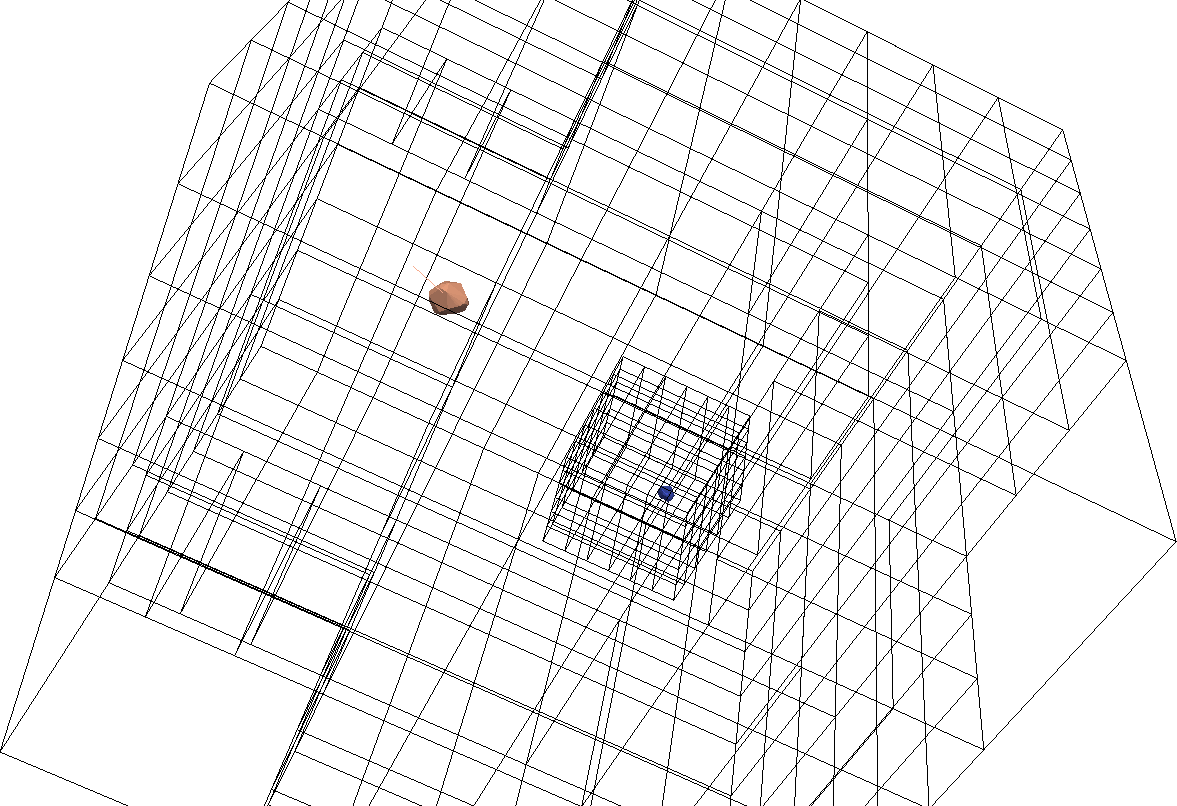
\includegraphics[width=0.4\textwidth]{experiments/two-bodies/visualisation/adaptive-grid00.png}
  \hspace{1.1cm}
  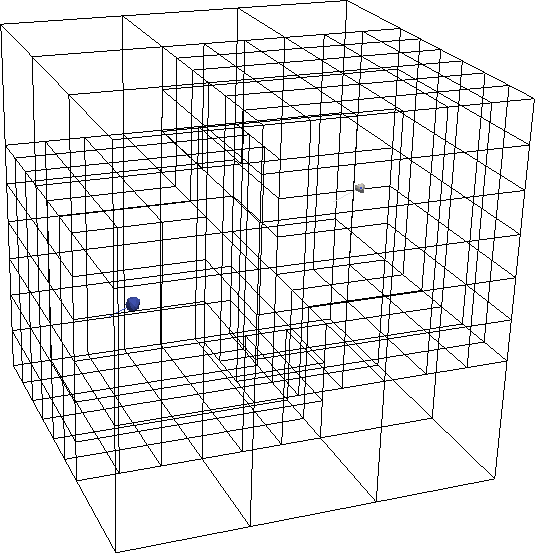
\includegraphics[width=0.25\textwidth]{experiments/two-bodies/visualisation/reluctant-adaptive-grid00.png}
  \\
  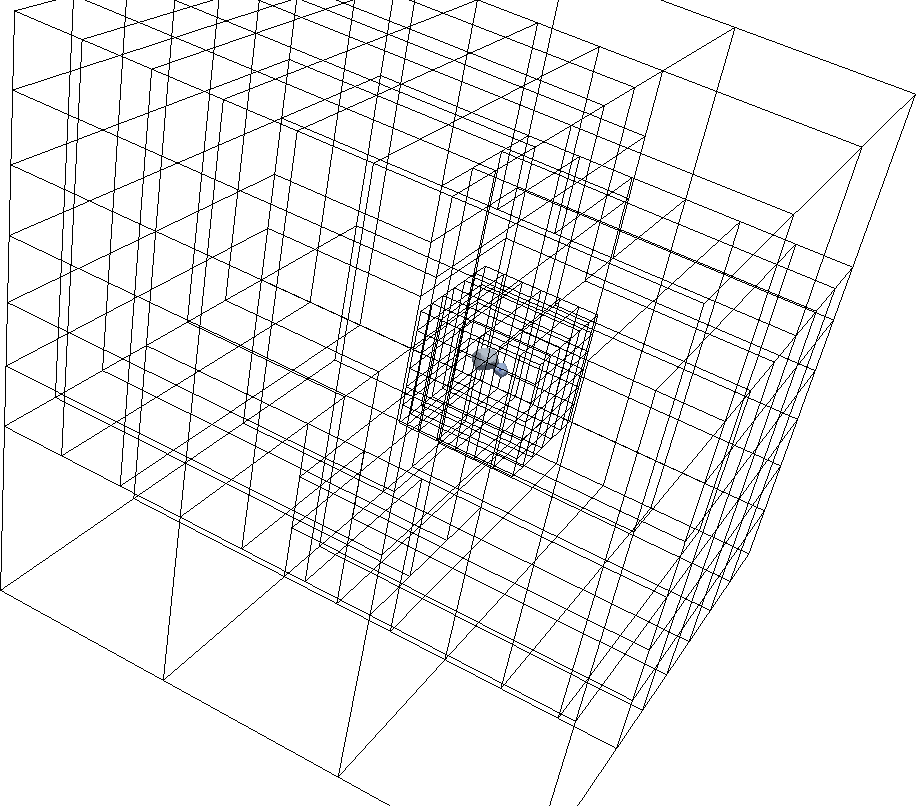
\includegraphics[width=0.3\textwidth]{experiments/two-bodies/visualisation/adaptive-grid02.png}
  \hspace{1.1cm}
  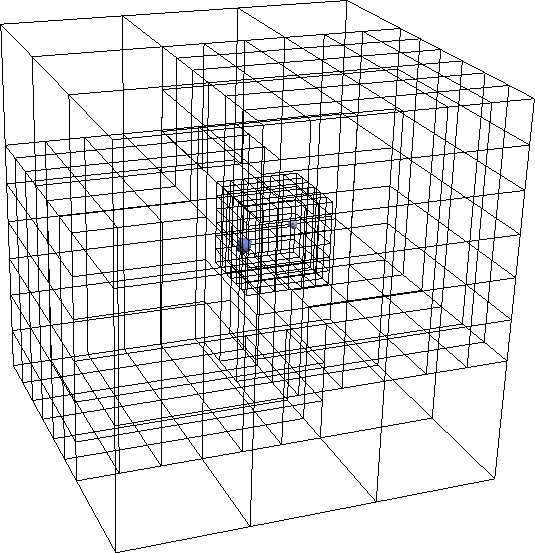
\includegraphics[width=0.3\textwidth]{experiments/two-bodies/visualisation/reluctant-adaptive-grid02.png}
% 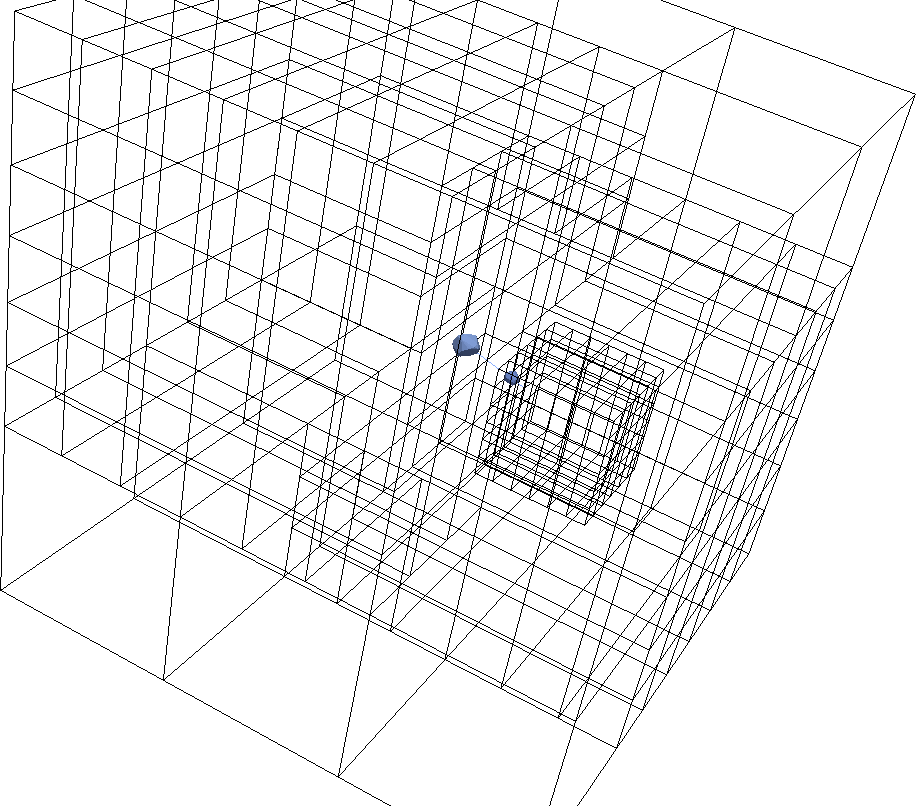
\includegraphics[width=0.3\textwidth]{experiments/two-bodies/visualisation/adaptive-grid01.png}
%   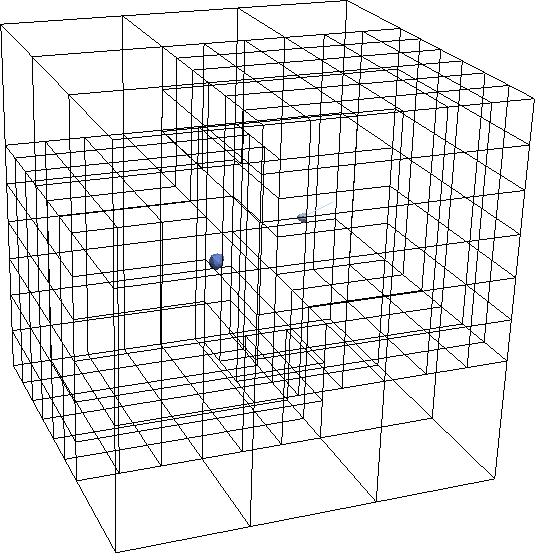
\includegraphics[width=0.3\textwidth]{experiments/two-bodies/visualisation/reluctant-adaptive-grid01.png}\\
%   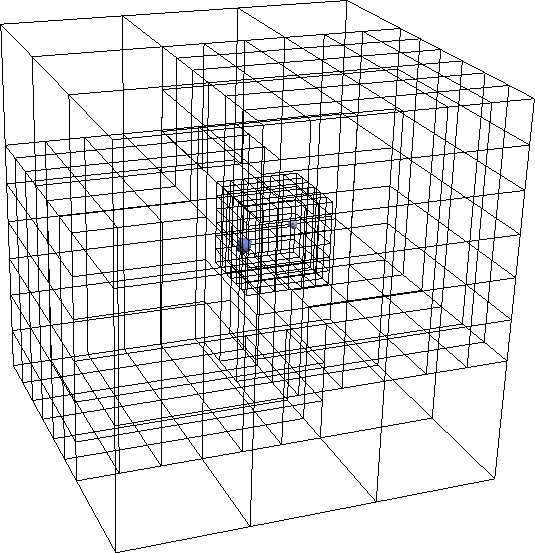
\includegraphics[width=0.3\textwidth]{experiments/two-bodies/visualisation/reluctant-adaptive-grid02.png}
%   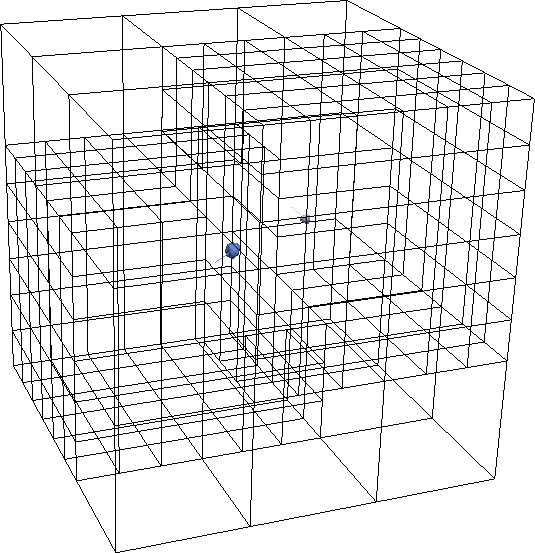
\includegraphics[width=0.3\textwidth]{experiments/two-bodies/visualisation/reluctant-adaptive-grid03.png}\\
 \end{center}
 \caption{
   Two particles crash into each other.
   The adaptive grid refining around each particle while its diameter
   constrains the mesh size (left column).
   The reluctant adaptive grid works with a coarser resolution as long
   as particles are far away from each other (right column).
   Just before they collide, the grid is refined and particles are dropped down
   the resolution levels.
 }
 \label{figure:adaptive-vs-reluctant-grid}
\end{figure}

We define two multiscale relationships between vertices (Figure
\ref{figure:collision-cube}).
A vertex $a$ is a child of a vertex $b$ if all adjacent cells of $a$ are
children of adjacent cells of $b$. $b$ is the parent vertex of $a$.
A vertex $a$ is a descendant of $b$ if at least one adjacent cell of $a$ is a
child of an adjacent cell of $b$. $b$ is an ancestor of $a$.
If we delete a vertex $a$ that holds particles, its particles are moved to the
next coarser level and assigned there to the nearest parent of $a$.
Each vertex holds a boolean marker that is set $\bot $ before the vertex is
read for the first time.
If a vertex holds a particle, all the markers of the vertices where it is a
descendent from are set to $\top$.
If a vertex whose adjacent cells all are refined holds $\bot$ at the end of the
multiscale traversal, we coarsen these refined adjacent cells.
We rely on a top-down tree traversal.
The refinement/coarsening procedure then can be evaluated on-the-fly.
It equals an analysed tree grammar \cite{Knuth71}.

For the multiscale contact detection, we extend the list of particles associated
to a vertex. 
There is the list of actually held particles and a list of virtual particles. 
We run through the grid top down, i.e.~a vertex always is read for the first
time before any of its descendants, and clear virtual particle list first.
Then, we add all particles held in the particle or the virtual particle lists of
any ancestor to the local virtual list.
If we compare all particles with each other that are held by the same vertex, we
do compare the actual particles with all other real particles as well as all
virtual particles.

{\bf A reluctant adaptive grid.}
The dynamically adaptive grid refines rather aggressive: Particles are always
dropped to their corresponing refinement level immediately. 
Fine grid regions thus follow 'their' particles (Figure
\ref{figure:adaptive-vs-reluctant-grid}).
This might introduce finer grids than actually required for contact detection
which is an overhead.
Given the one-cell-per-time-step constraint on the particle velocity, we also
restrict the maximum velocity or time step rigorously.
For the present work, this does not have a major impact as we apply uniform
small time step sizes globally. 
For schemes with local time stepping, it however is important, besides overhead
discussions, to keep the grid as coarse as possible as this facilitates big
time step sizes.

Our reluctant adaptive grid works with coarser adaptive grids than the plain
variant through two modifications of the refinement procedure: 
On the one hand, we refine the region around a vertex if the previous criterion
holds and the vertex holds at least two particles.
If only one particle is holds, we stick locally to the grid no matter what the
particular diameter is.
Throughout the inter-vertex contact detection in \texttt{enterCell}, we further
bookkeep the minimum diameter of all the particles involved. 
If this minimal diameter is smaller than the cell, we do refine this cell, too.


\section{Shared memory parallelisation}
\label{section:shared-memory}

We introduce three levels of shared memory parallelisation on a single machine that exploit multiple levels of locality. The hierarchical categorisation of the methods is based upon the abstract algorithmic distance between shared resource parallel utilisation and actual arithmetic computation. At the highest level we exploit  data access independence of vertex touches we assign cell block tasks to threads. Within each vertex touch particle pairs are grouped into aligned memory blocks thus tasks are launched between particle-to-particle comparisons. Lastly within each particle pair at the innermost level tessellation elements of the mesh are dichotomised and parallel locality is held for the underlying vectorized contact solver.

Three levels of multicore parallelisation:\\

a) cell level cell-to-cell thread units\\

b) cell vertex level particle-to-particle thread units\\

c) particle level mesh-to-mesh thread units\\

%describe the setup
We utilise particles approximated by a random spherical point cloud, arbitrary particle surfaces are generated with the Delauny triangulation algorithm. The algorithm is scaled in three respects; number of non-spherical particles, irregularity of particle radius size, and mesh size. Respectively, we provide three parameters in the creation of the simulation domain. $Rmin$, $Rmax$ parameter for max and min radius of particles, $m$ for mesh density, $p$ for number of particles in the domain. These allow observation of the interplay between performance and particle geometry and dynamics within a grid in a modern NUMA architecture. For scaling measuring we use the hybrid and the brute force solvers.

%Initial-termination conditions
For the experiment the initial space configuration of the particles in respect to the grid is homogeneous and aligned per cell. Initial conditions for the particle dynamics are governed by only gravity and termination is defined by the number of iteration that the granulates are rest condition with energy dissipated on the ground. Termination phase is known a priori. We utilise regular grid and reluctant-adaptive grids for space decomposition and and grid adaptivity to granular kinematics. 

\iffalse
\begin{figure}[htb]
	\centering
	\begin{subfigure}{.5\textwidth}
  		\centering
    	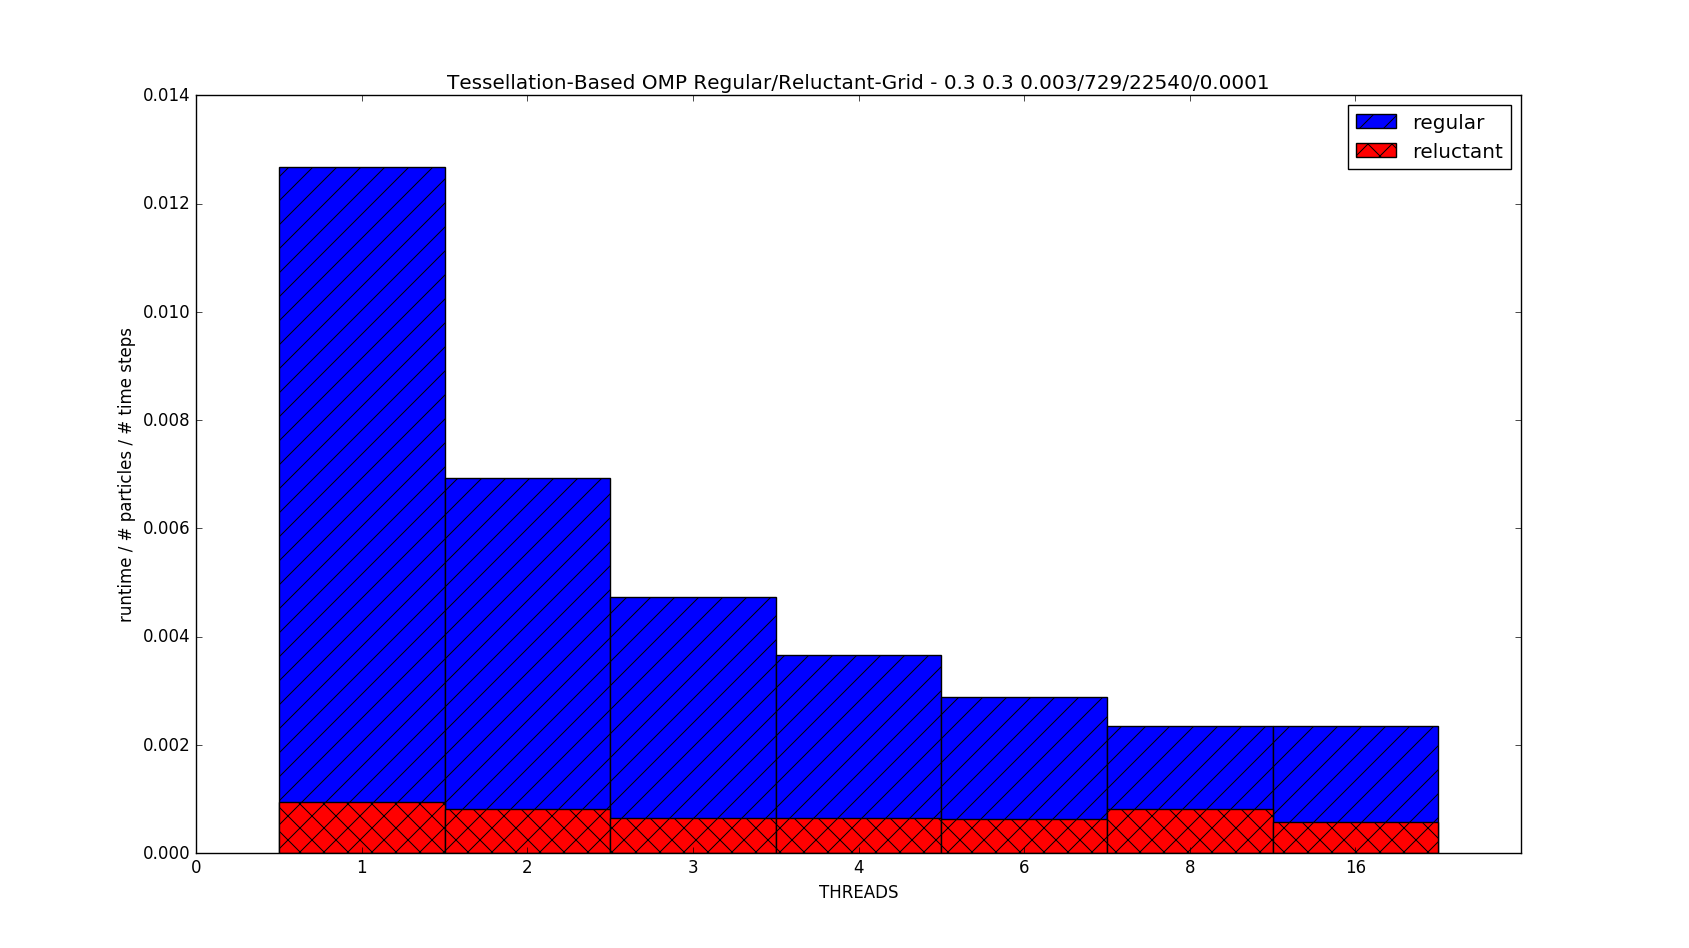
\includegraphics[width=1\textwidth]{experiments/omp/omp_mesh_regular-reluctant_20.png}
  		\caption{Shared memory scaling 22540 elements.}
  		\label{figure:omp_regular_reluctant_triangle_200}
	\end{subfigure}%
	\begin{subfigure}{0.5\textwidth}
  		\centering
    	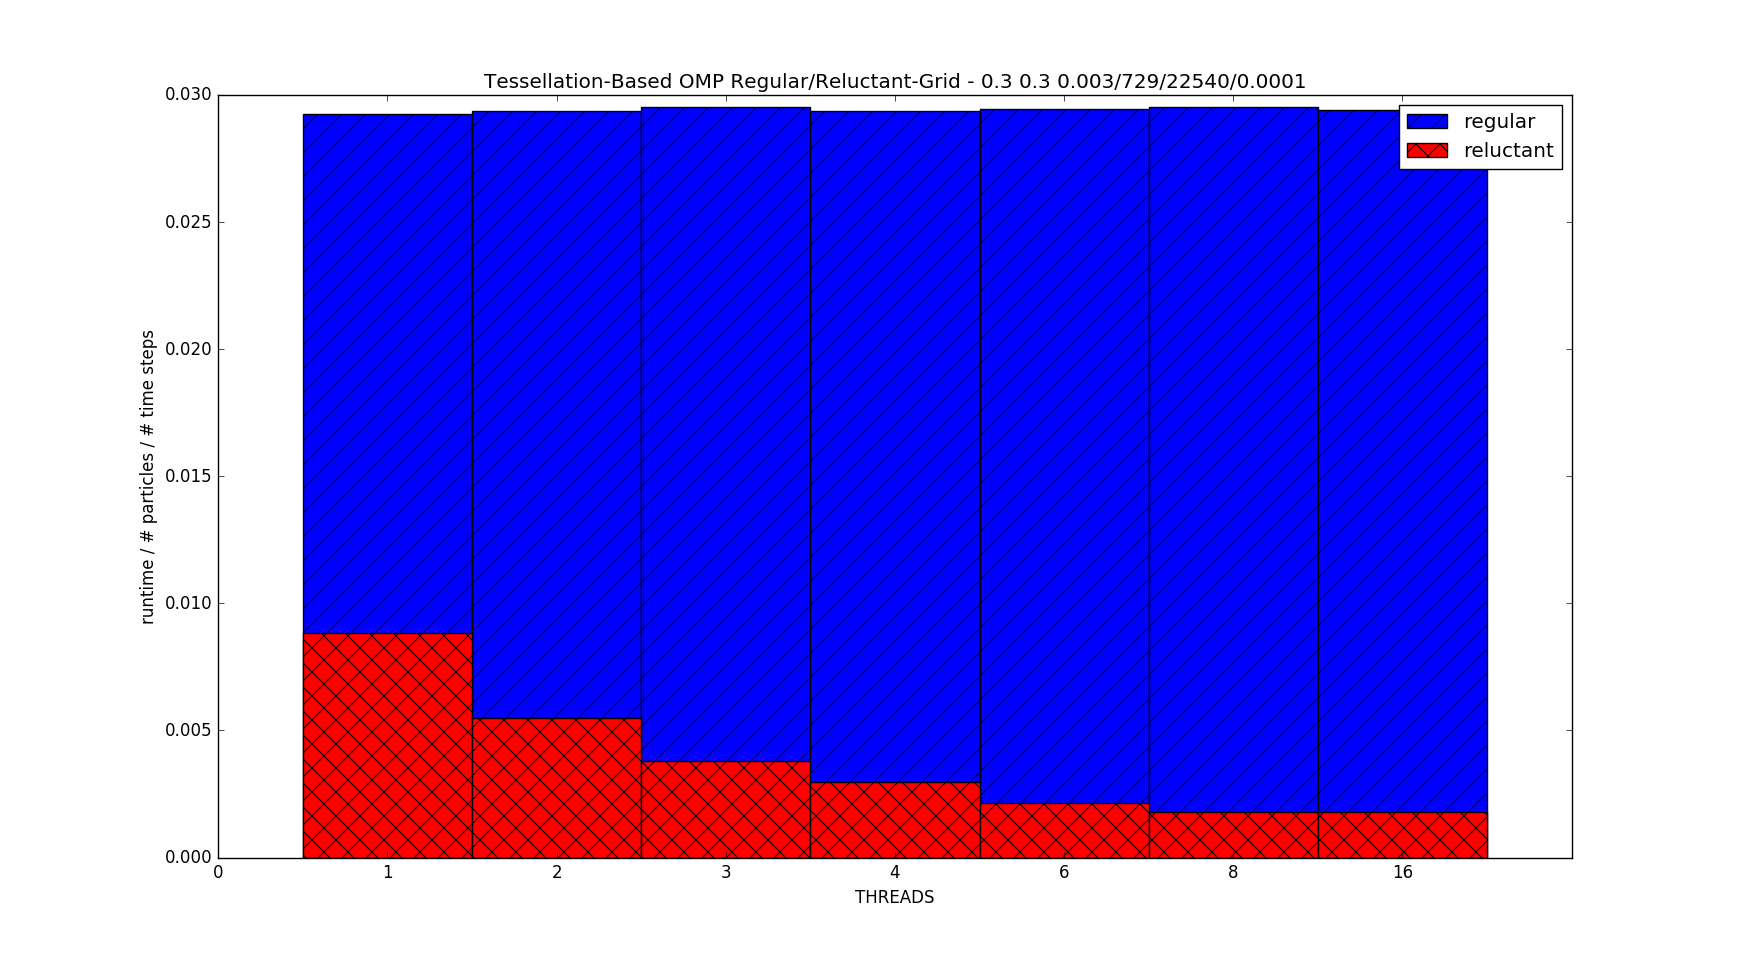
\includegraphics[width=1\textwidth]{experiments/omp/omp_mesh_regular-reluctant_200.png}
  		\caption{Shared memory scaling 98540  elements.}	
  		\label{figure:omp_regular_reluctant_triangle_200}
	\end{subfigure}
\end{figure}
\fi

\begin{figure}[htb]
  \begin{center}
    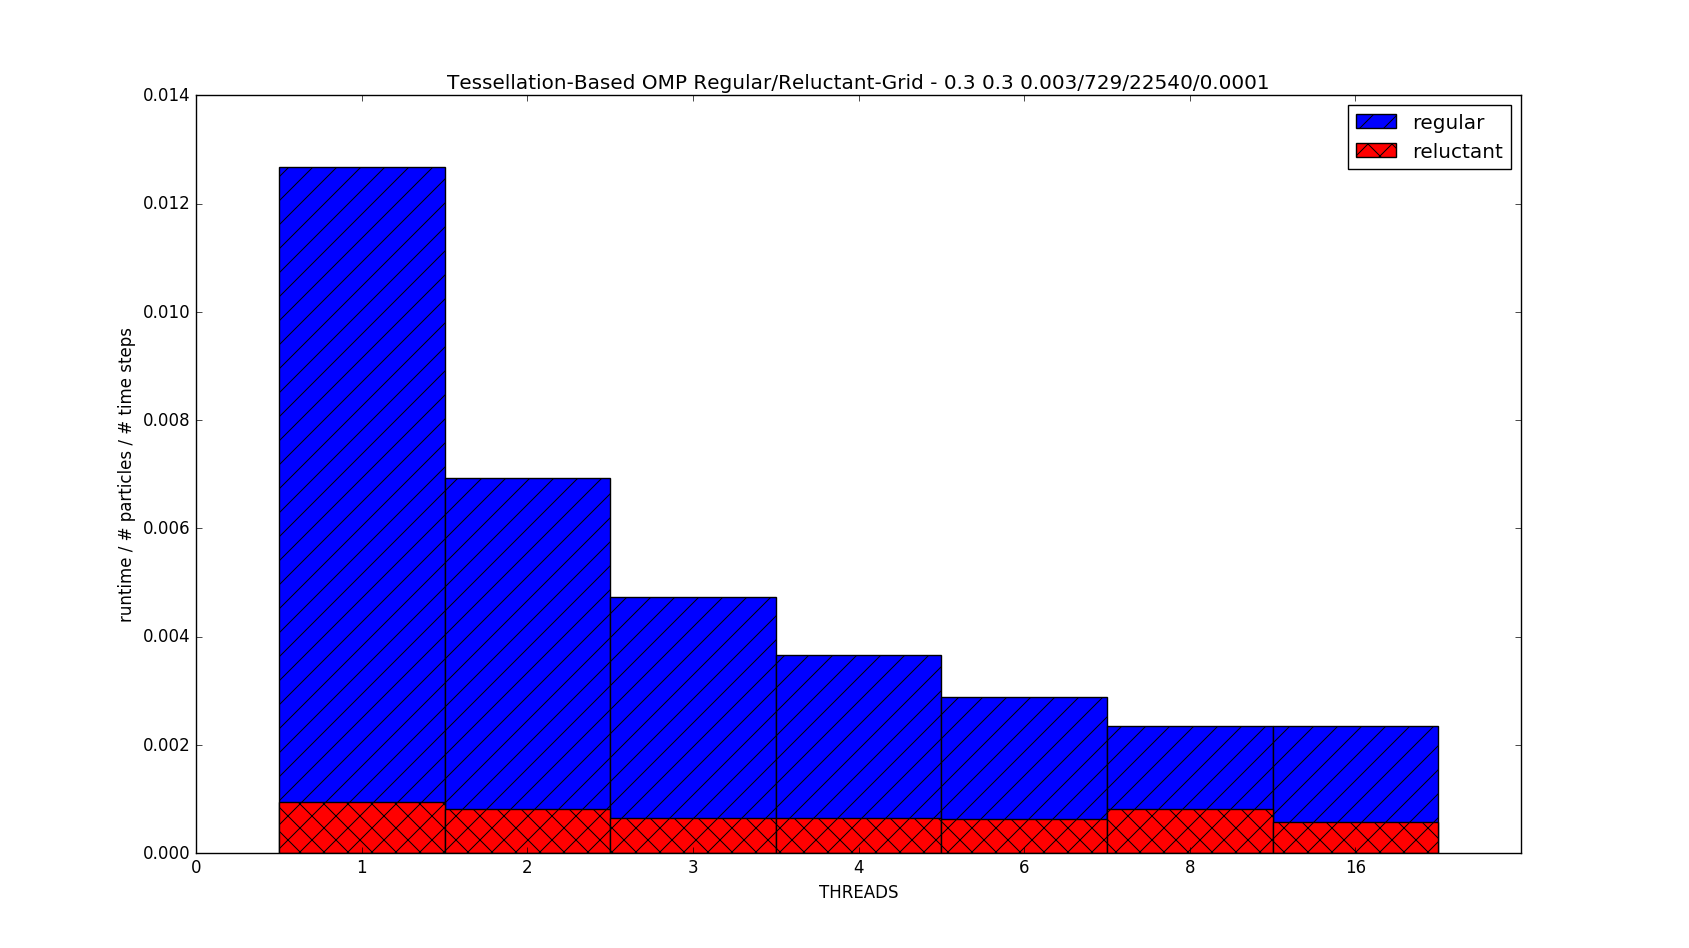
\includegraphics[width=1\textwidth]{experiments/omp/omp_mesh_regular-reluctant_20.png}
  \end{center}
  \caption{Grids shared memory scaling 22540 triangle elements (BF solver).}
  \label{figure:omp_regular_reluctant_triangle_20}
\end{figure}

\begin{figure}[htb]
  \begin{center}
    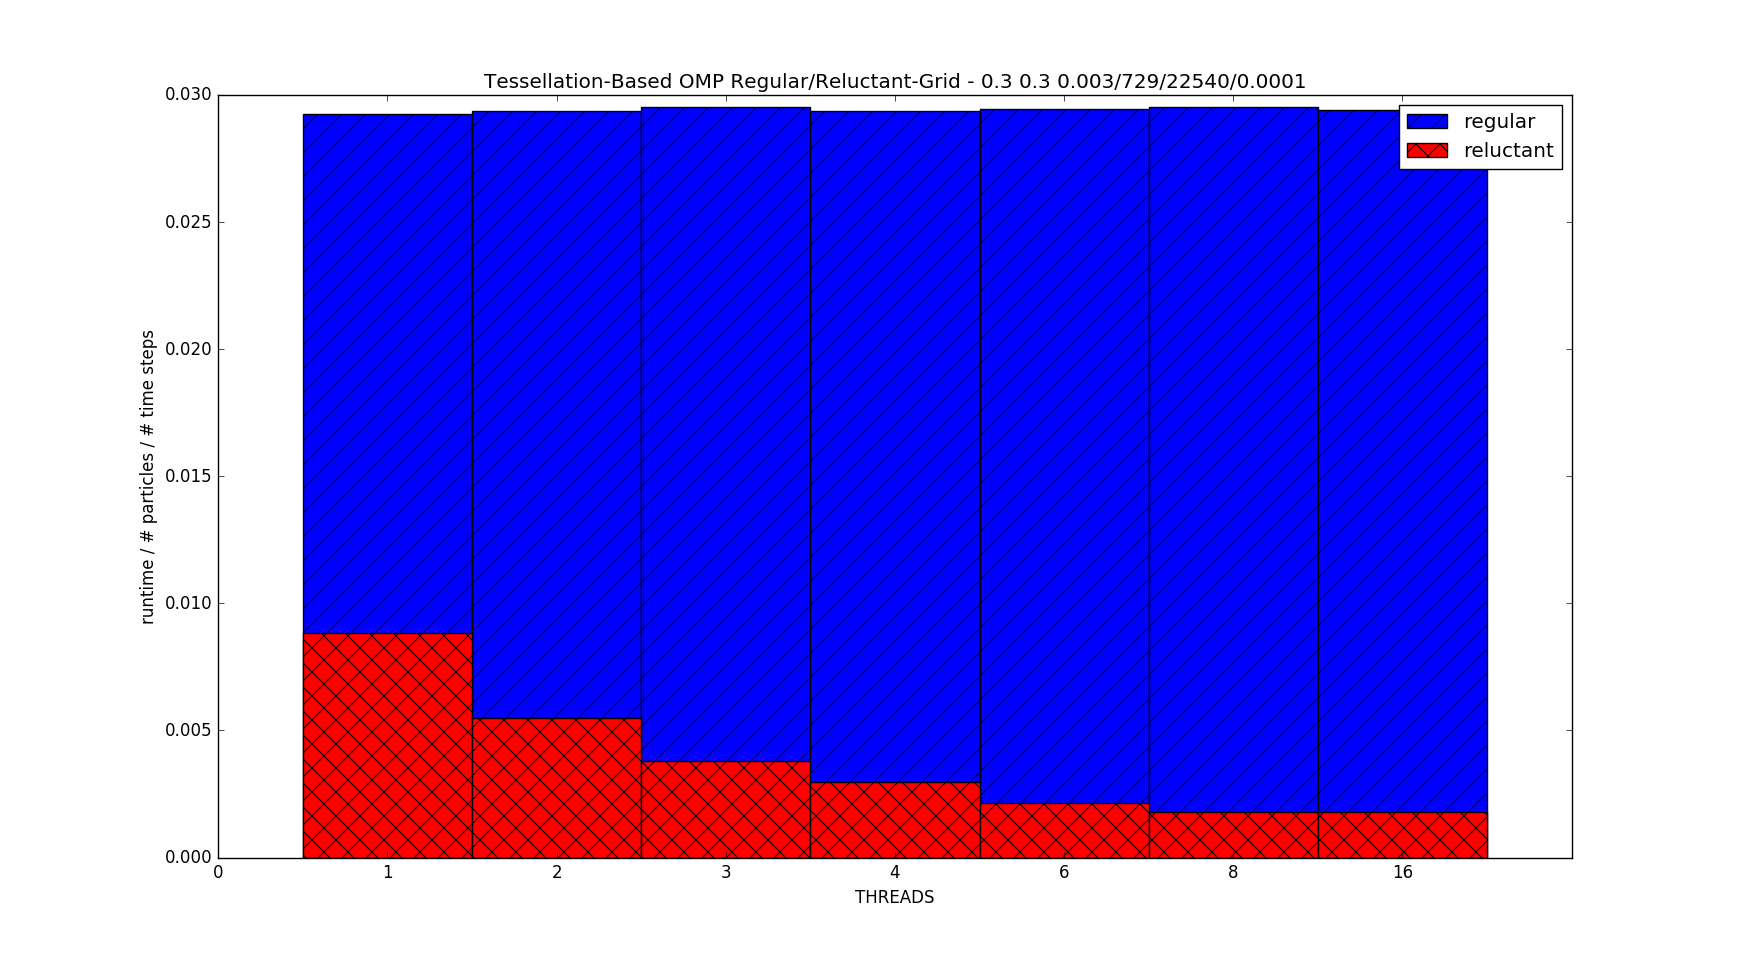
\includegraphics[width=1\textwidth]{experiments/omp/omp_mesh_regular-reluctant_200.png}
  \end{center}
  \caption{Grids shared memory scaling 98540 triangle elements (BF solver).}
  \label{figure:omp_regular_reluctant_triangle_200}
\end{figure}


%STEP A
Beginning at the innermost tessellation-level with a regular grid (figure \ref{omp_regular_reluctant_triangle_20}) on a NUMA ivy bridge system the code scales linearly up to the eight-core single die. As the size of the problem increase for weak scaling (figure \ref{omp_regular_reluctant_triangle_200}) the computation to memory bandwidth rate ratio is no longer sustainable computation to scale over multiple cores. Similarly on a small computational domain (figure \ref{omp_regular_reluctant_triangle_20}, blue) with minimum weighted threads grid adaptivity doesn't pay off as thread initialisation, scheduling, grid adaptivity and memory access overhead dominates over arithmetic intensity. Contrary to regular grid, adaptivity allows up-scaling towards both increasingly larger computations (figure \ref{omp_regular_reluctant_triangle_200}) and number of cores as long as bandwidth, compute bounds are not reached or thread overheads are not the bottleneck. In all cases the brute force solver does not scale pass the second die interconnect as communication to memory stagnates.

\begin{figure}[htb]
  \begin{center}
    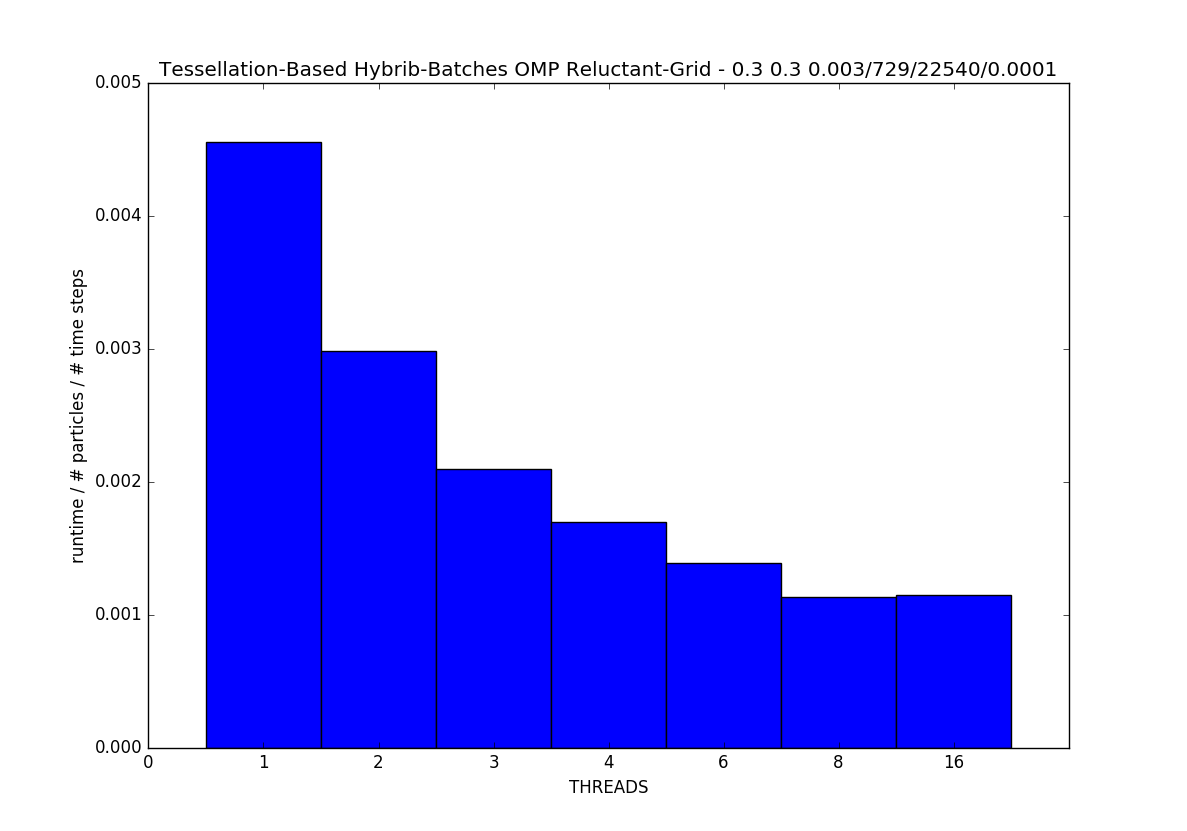
\includegraphics[width=0.8\textwidth]{experiments/omp/hbatches_omp_triangles_200.png}
  \end{center}
  \caption{Triangle based shared memory running hybrid-on-batches (HBatches).}
  \label{figure:hbatches_triangles_triangle_omp}
\end{figure}

Arithmetic, bandwidth intensity and data access patterns vary among solvers in the innermost level and can yield different performance results. The hybrid solver is parallelised in two different hybrid schemes triangle-to-triangle pairs and triangle-to-triangle batches, both launch different types of threads. For the hybrid-on-batches solver the tessellation-based threads
are $n$ triangle batches wide while hybrid-on-triangles solver relies on fine couples of threads. The non-deterministic nature and error-prone distribution of triangles of the hybrid algorithm as discussed in Chapter {-hybrid chapter-} would suggest that alternative scheduling would pay off. But for our experiments dynamic and guided thread scheduling don't have a performance gain but they rather create scheduling overhead due to error distribution in triangle pairs and due to the granularity of our batches. For the hybrid-on-triangles that is also the case because although the arithmetic intensity is dense in the solver, it doesn't last long enough to significantly overlap the cost of threading overhead. 

\begin{figure}[htb]
  \begin{center}
    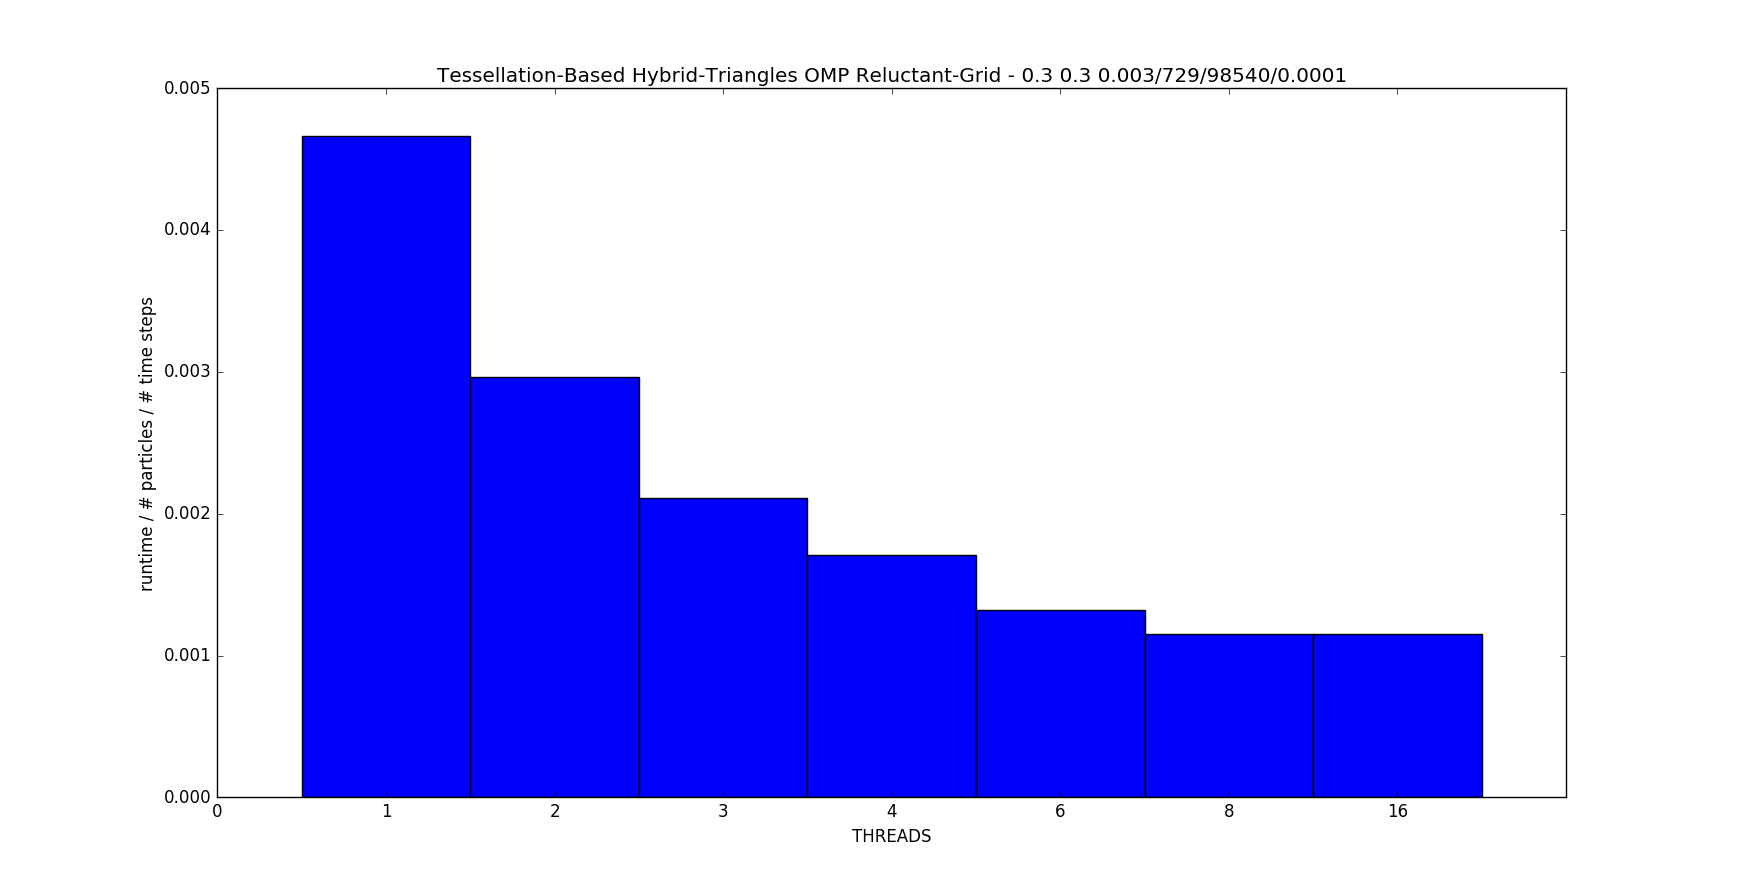
\includegraphics[width=0.8\textwidth]{experiments/omp/htriangle_omp_triangles_200.png}
  \end{center}
  \caption{Triangle based shared memory running hybrid-on-triangle-pairs (HTriangles)}
  \label{figure:htriangles_triangles_triangle_omp}
\end{figure}


\begin{figure}[htb]
  \begin{center}
    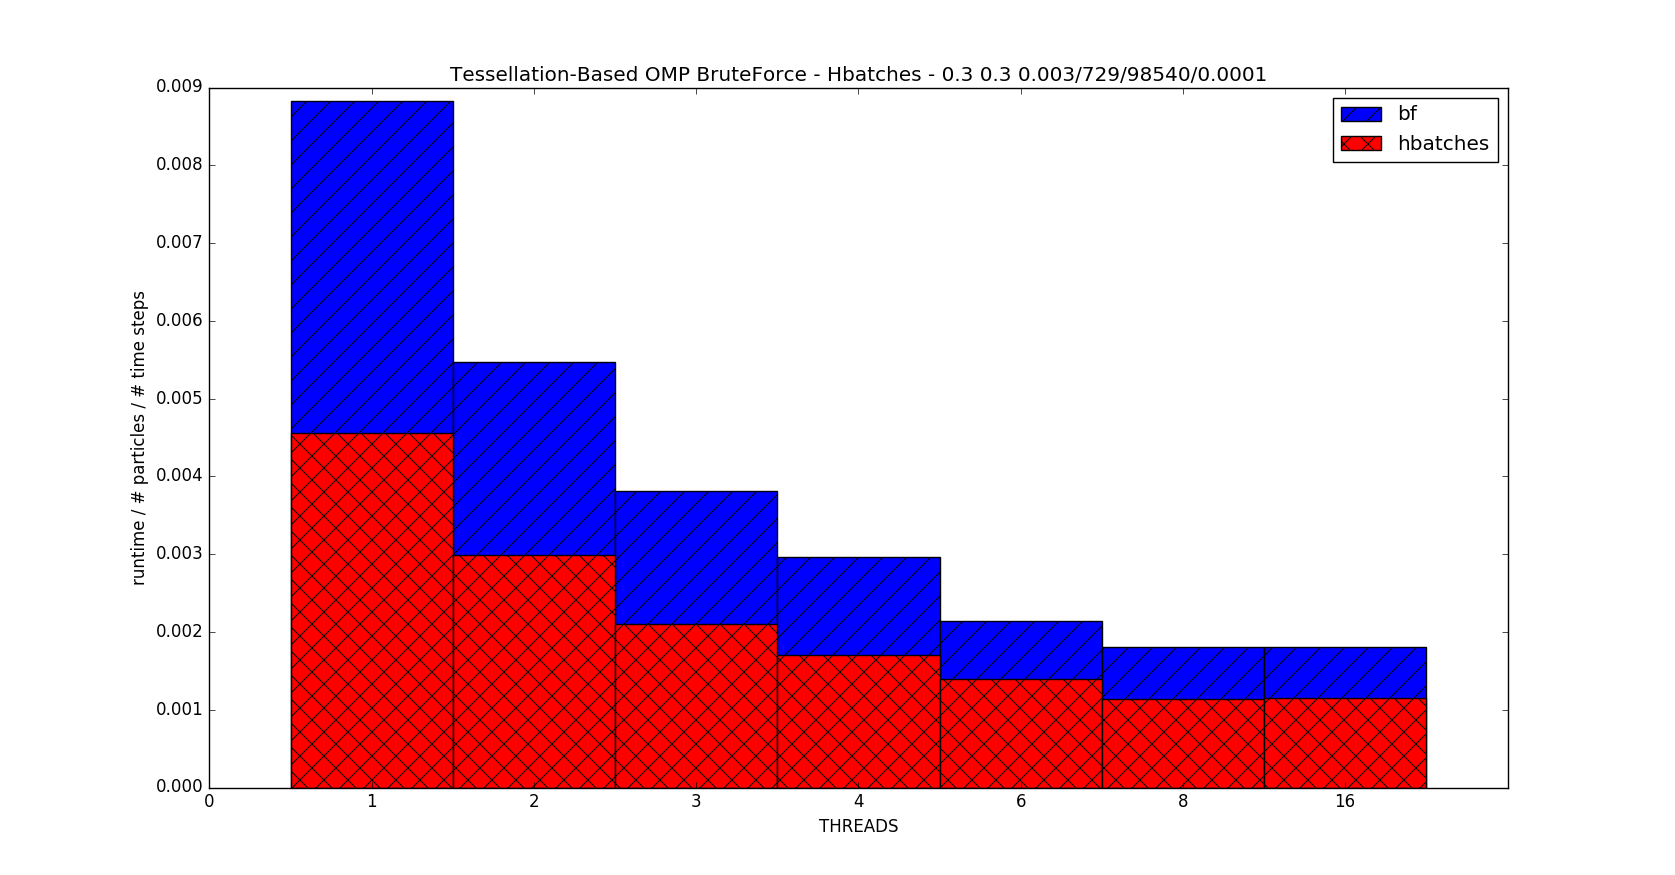
\includegraphics[width=0.8\textwidth]{experiments/omp/bf_vs_hbatches_omp_200.png}
  \end{center}
  \caption{Triangle based shared memory running hybrid-on-triangle-pairs (HTriangles)}
  \label{figure:bfvshbatches_triangle_omp}
\end{figure}

Figure \ref{figure:hbatches_htriangles_triangle_omp} hybrid-on-triangle and hybrid-on-batches scales up to eight cores on the single dice but also neither gain from offloading to the second socket. In practice hybrids normalized time to solution is significantly greater than brute force as seen in Figure \ref{bfvshbatches_triangle_omp}

%VITUNE results and memory bandwidth compared to stream.  

%STEP B

At the outer parallel blocks, particle blocks are threaded within each grid-vertex touch. In Figure \ref{figure:particle_omp} brute force does not scale at all and that is due to the adaptive domain decomposition and not due to the solver. The aggressive particle decomposition per grid cell since the preconditioning of the simulation creates a access pattern contradiction to the dense tile access patterns that tessellation method exploits. The overhead and the precondition enforced by the grid for minimum number of particles per vertex doesn't allow any scaling to occur on any method. Particle density is too low for thread launching and compute-wise scaling, memory communication overtakes the simulation time. 

\begin{figure}[htb]
  \begin{center}
    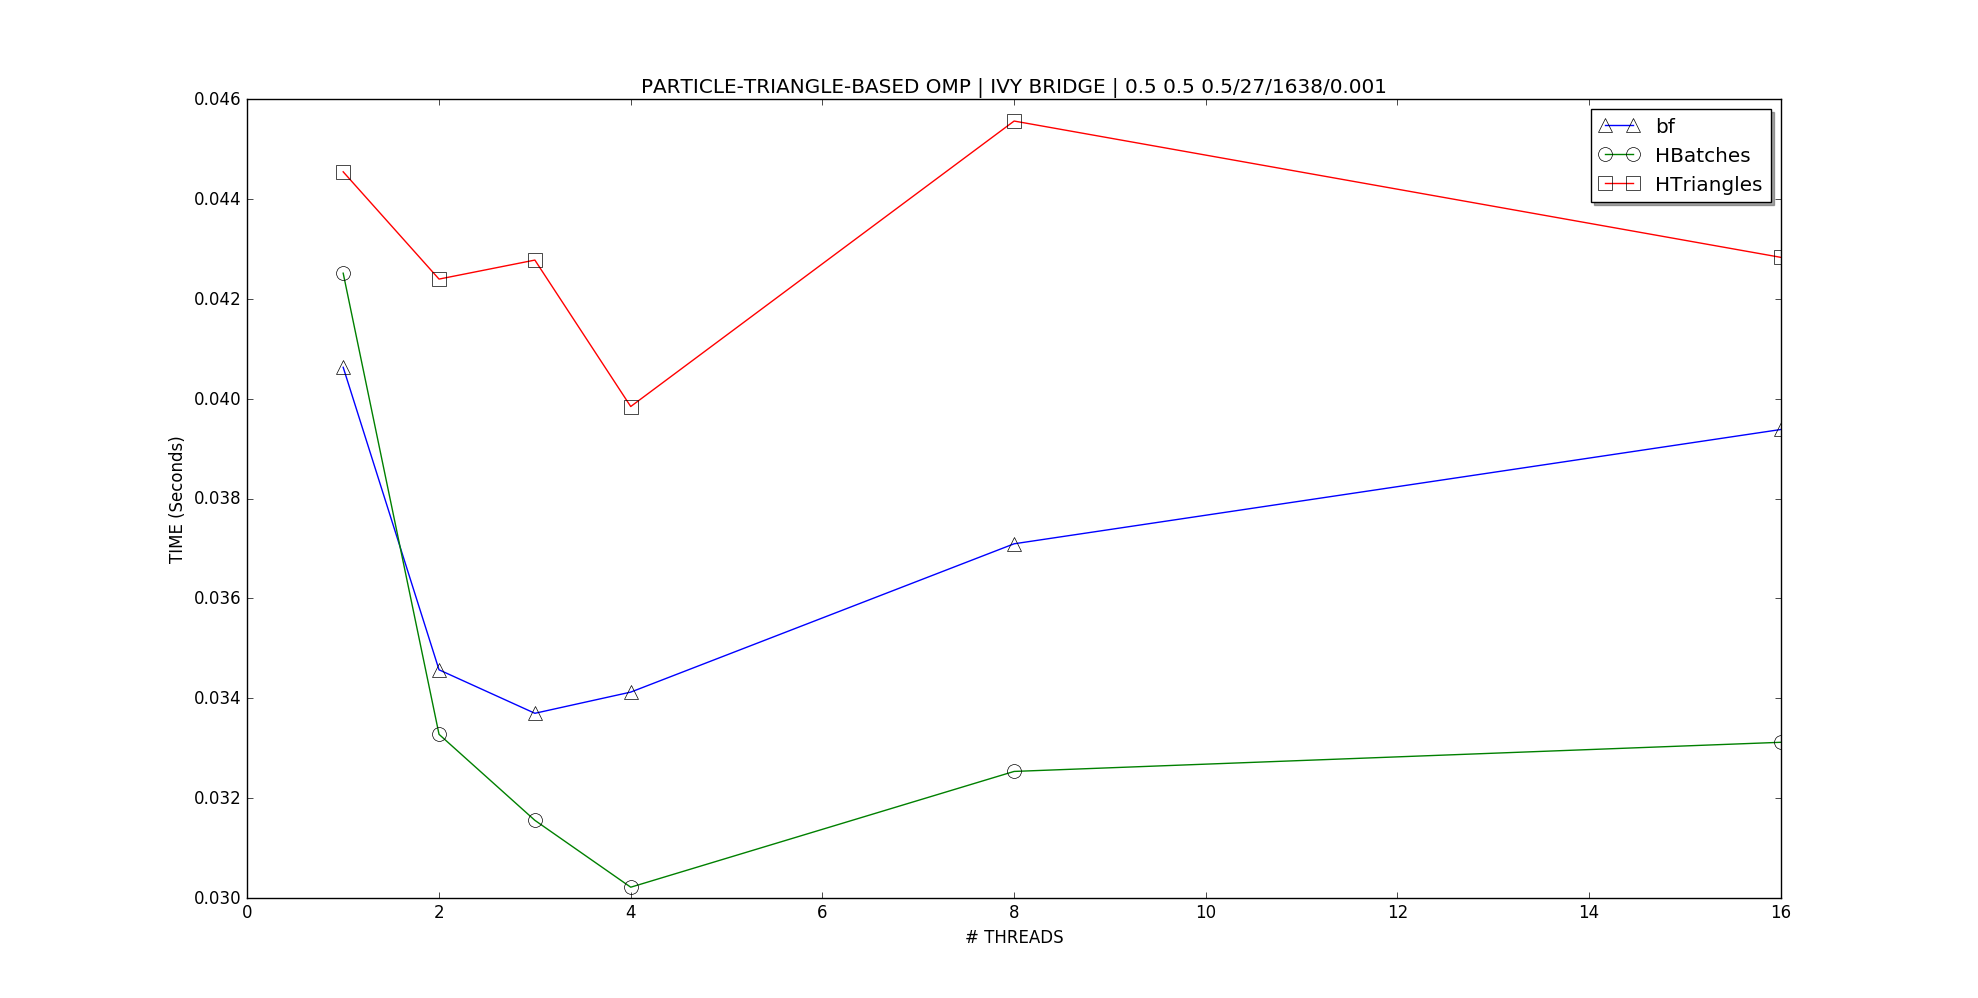
\includegraphics[width=1\textwidth]{experiments/random/omp/particle_triangle_based_x0.png}
  \end{center}
  \caption{Particle based nested shared memory brute force (bf)}
  \label{figure:particletriangle_omp}
\end{figure}

%Particle and Triangle parallelism nests both particle and triangle shared memory threads. The runtime to solution is slightly slower than particle-based parallelism due to overhead. 

%Nevertheless it has an impact on brute-force method as it scales smoother than particle-based only parallelism due to overhead. In this case hybrid-on-batches is also the fastest while the hybrid-on-triangle-pairs the slowest. 


%STEP C

\begin{figure}[htb]
  \begin{center}
    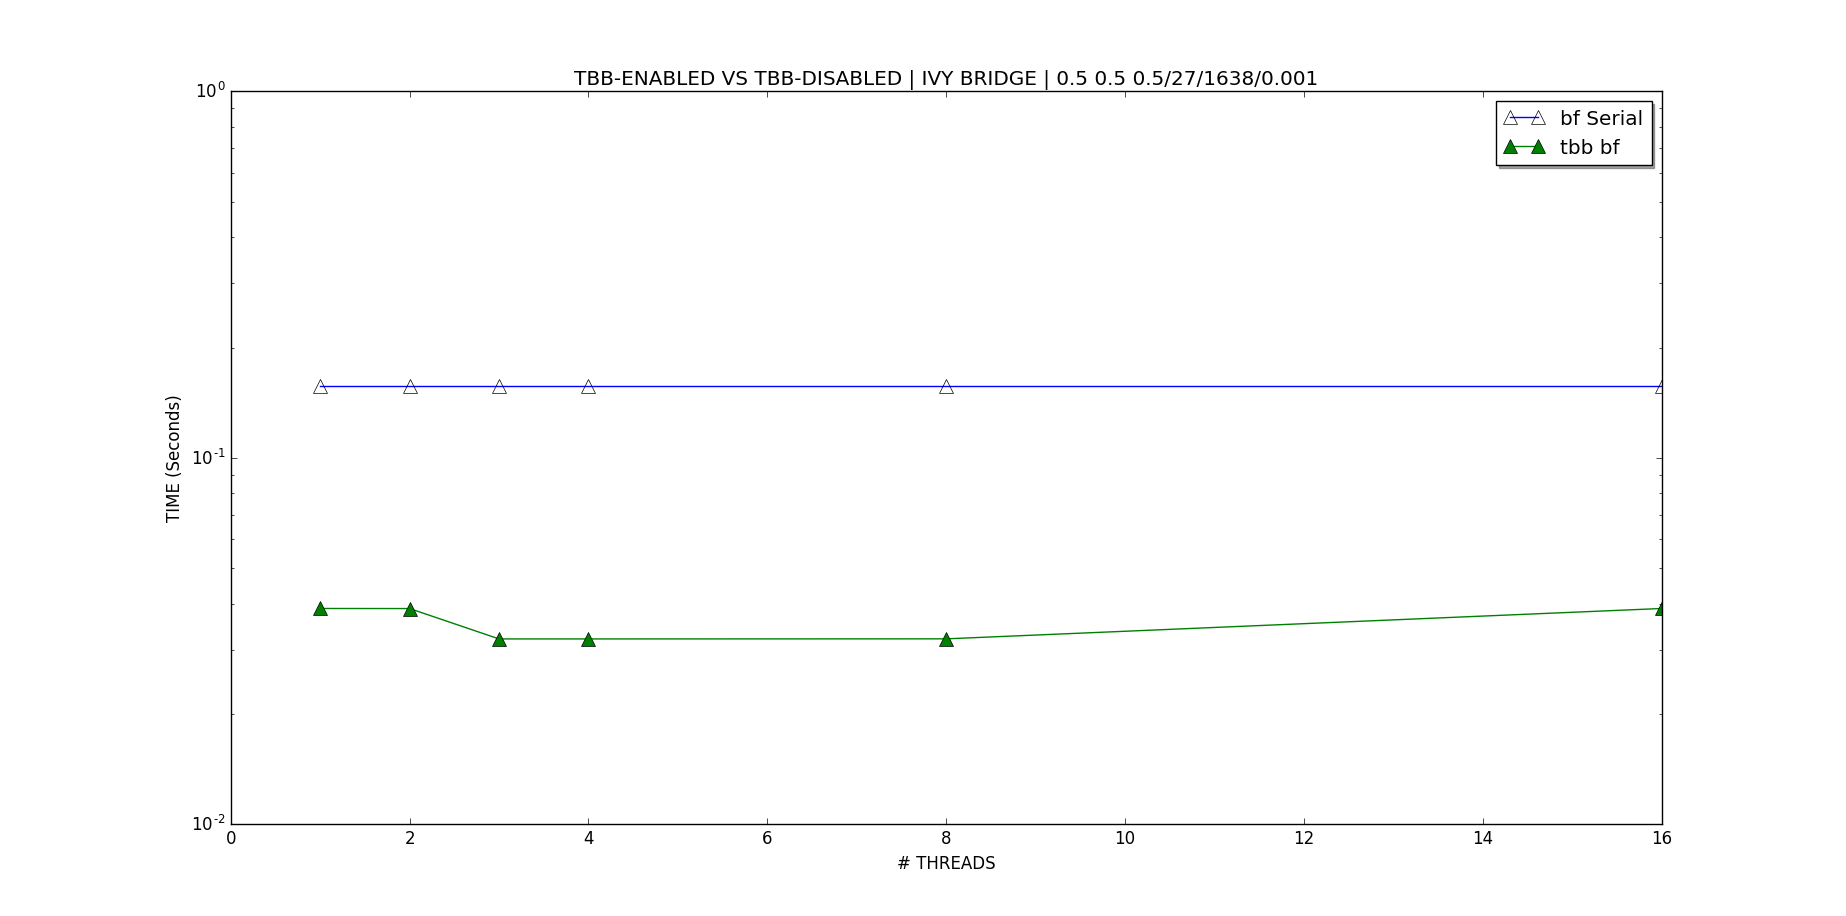
\includegraphics[width=1\textwidth]{experiments/random/omp/tbb_vs_serial.png}
  \end{center}
  \caption{Cell based parallelism on Peano compared to serial runs using Intel TBB}
  \label{figure:tbb_vs_serial}
\end{figure}
  

At the highest level of shared memory parallelism is the grid cell-based multicore processing. It is based on the peano-framework that is using Intel TBBs to assign cells on threads. This has significant impact on the overall runtime performance in Figure \ref{figure:tbb_vs_serial} it is compared with plain serial execution. Number of threads on the x axis refer to TBB Cell-based threads, at the contact detection method level the computation is performed without shared memory parallelism but with vectorization enabled. For the specified experiment in Figure {} we observe no cell-based thread scaling but only reduction of time to solution. But when we increase the problem size further (figure \ref{figure:tbb_scaling}) we see that cell-based parallelism scales and it enhances execution time. 

\begin{figure}[htb]
  \begin{center}
    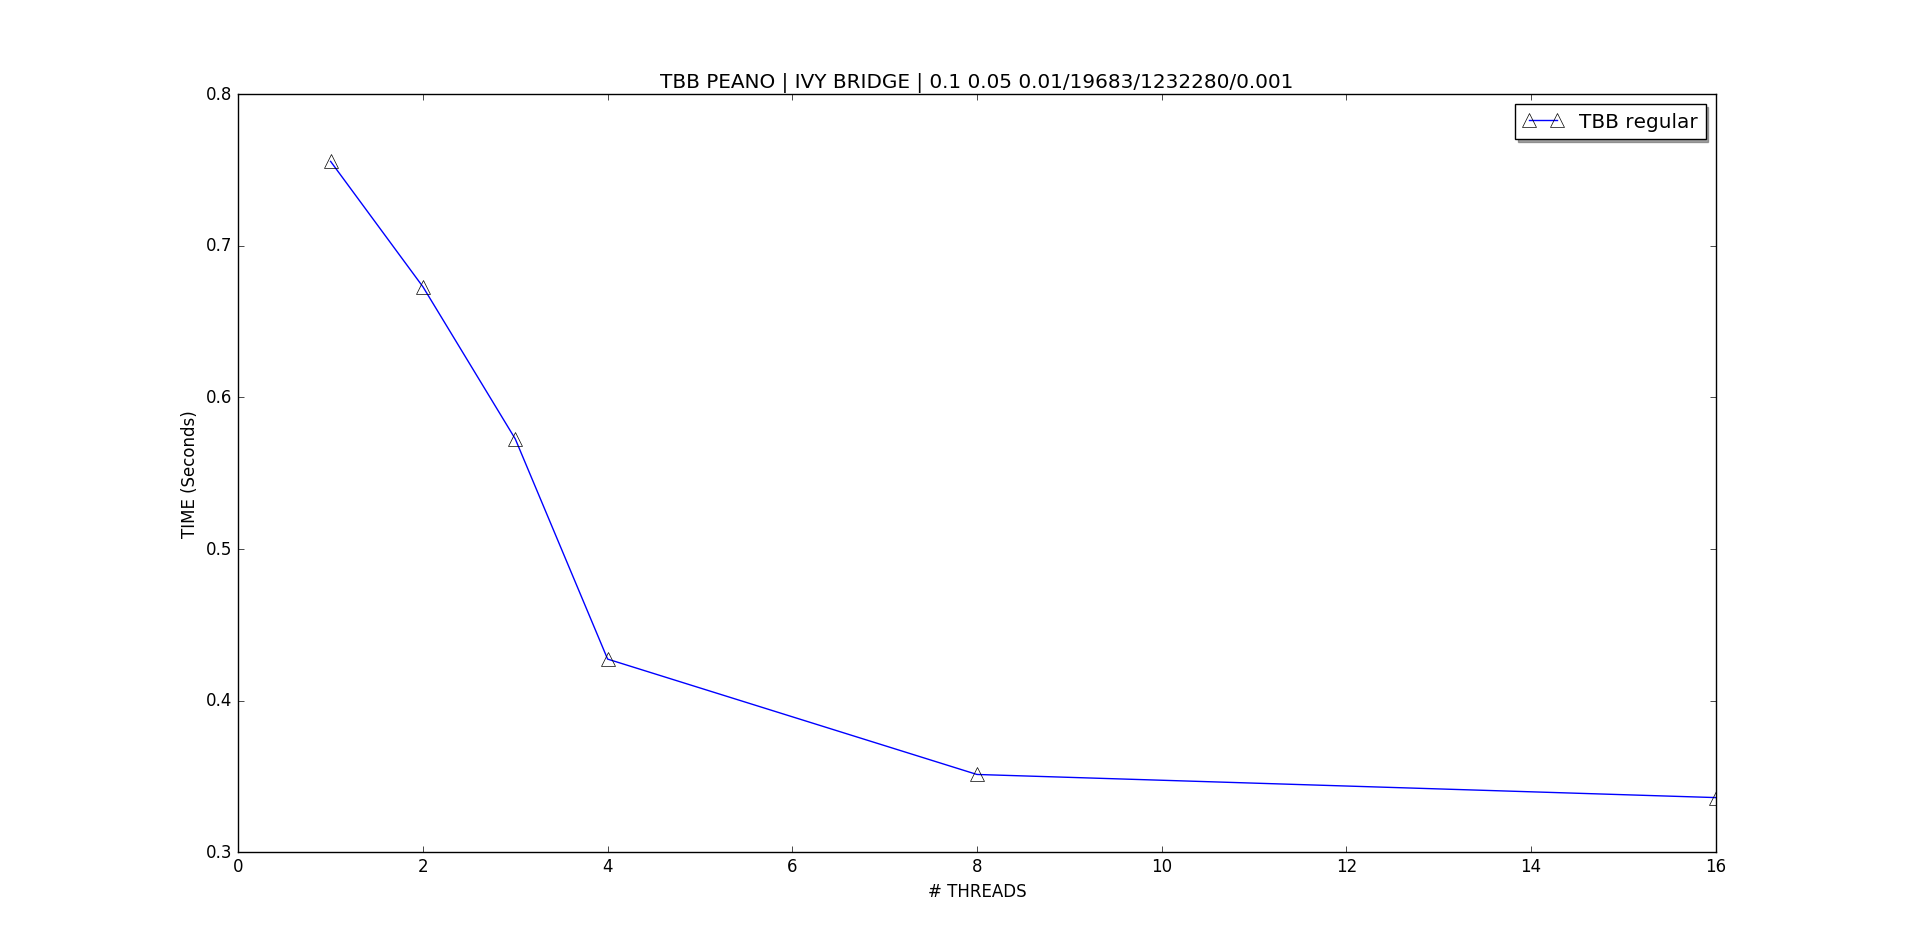
\includegraphics[width=0.8\textwidth]{experiments/random/omp/tbb_regular_x2.png}
  \end{center}
  \caption{Cell based parallelism on Peano compared to serial runs using Intel TBB}
  \label{figure:tbb_scaling}
\end{figure}

Overall shared memory parallelisation yield good speed ups both for hybrid and brute force using adaptive grids with triangle-based parallelism show good time-to-solution For large problem sizes the combination of cell-based plus triangle-based parallelism using hybrid-on-batches is the preferred option. Additional speedup can be gained if spheres are used as a filtering bounding box stage to our triangle-to-triangle contact detection.

\clearpage




\section{Domain Decomposition for Contact Detection}
\vspace{5mm}
\begin{itemize}
\item Completed since last report: Implemented domain decomposition for distributed memory load balancing using library, MPI blocking communication for data migration. 
\item New concepts: Overlapping process communication for contact detection with ghost data. Asynchronous communication waiting
time significant as number of ranks increase.
\item Open questions: multilayer grid/spacetree implementation for DEM 
\end{itemize}

We further scale the computation of triangle-to-triangle contact with the Message Passing Interface (MPI) \cite{Forum:1994:MMI:898758} for distributed memory computation. Our DEM-based contact detection is inspired by molecular dynamics simulations, where millions of spheres are simulated. State-of-the-art MD computation is decomposed into smaller computational sub-domains and communication exchanges necessary boundary information. Similar computational stages are applied by us in the DEM-based contact detection algorithm. We study synchronous and asynchronous modes of data exchange and how two communication strategies can be exploited to increase performance and minimize computation.

The distributed memory DEM contact detection algorithm is performed in three stages. In stage one the computational domain is divided into equally balanced sub-domains. In stage two, data migration assigns the sub-domains to MPI instances. In stage three, we compute the distances to determine contact between all triangles. In stage four we accumulate the forces and in stage five we perform the explicit time step integration.

To scale the performance of contact detection simulation, the computational workload has to be processed in parallel by splitting the domain into sub-domains and computation deployment is based on it, making the decomposition an important stage. Decomposition affects load balancing and the communication patterns of the simulation. Communication is essential when sub-domains are inter-dependent since new boundaries are introduced with decomposition. It is important to decompose evenly whilst also reducing sub-domain communication. There are three types of decomposition that are widely used in different contexts \cite{Eckhardt2014, Plimpton1995} that can apply in DEM. Decomposition by particle, decomposition by force and spatial decomposition. 

In domain decomposition by particle \cite{koziara2011}, the domain is divided such that all sub-domains hold equal number of particles. For N particles we split the domain to N parts and we assign them to P processors (N/P). The sub-domain boundary is always located at the space between particles. In this method an all-to-all communication is required to detect contact points because they are always located at the sub-domain boundary. The global communication is a major disadvantage for small particles as each processor communicates with all other processors, staggering the overall parallel processing. Another disadvantage is the non-equal splitting (N/P) as some particles may require more computation than others (i.e. more triangles). The main advantage of particle-based decomposition is the implementation simplicity \cite{Plimpton1995}.

An alternative decomposition approach found in literature is force-based decomposition that is often applied in molecular dynamics (MD) and smoother particle hydrodynamic (SPH) simulations \cite{Bowers2007, Gaburov, Gonnet2014, Plimpton1995, Rycroft2012, Shaw2005}. The method formulates a interaction force matrix that solves the contact detection and the forces as a group of linear equations. The matrix is decomposed into small blocks and shared on each process to solve in parallel. Force based decomposition assume short-range interactions and thus a dense force matrix to solve. In force based methods, the advantage is that computation is decomposed without any spatial information from the particles. The major disadvantage in DEM applications is the assumption of dense and uniform sparse force matrices, the assumption can be wrong leading to imbalanced domains on run-time.   

According to N-body simulation literature \cite{Eckhardt2014, Fleissner, Wachs2012a, zomorodian2002} the state-of-the-art method for supercomputing applications is the spatial decomposition. Our decomposition is based on the spatial position of vertices using Recursive Coordinate Bisection (RCB) \cite{ZoltanIsorropiaOverview2012}. In RCB, the computational domain is first divided into two regions by a cutting plane orthogonal to one of the coordinate axes so that half the work load is in each of the sub-regions. The splitting direction is determined by computing in which coordinate direction the set of objects is most elongated, based upon the geometric locations of the objects. Each triangle vertex thus is owned and persistently stored exclusively on one process/sub-domain for the whole duration of the timestep. 

Spatial decomposition implicitly creates logical boundaries that split space and computation (c.f. Figure \ref{fig5}). The contact detection complexity of N trianglesthat belong to $n_{i}$ particles without boundary boxes is $\sum\limits_{i=0}^n n_{i}$ = O($n^2$) in big-O notation (Algorithm \ref{alg1}). Contrary, with equally spaced boundary boxes/cells, if C is the maximum number of particles then there are $26$ neighboring cells and $max(n_{i})$ is the maximum number of triangles per particle i which result to $n_{1} \times 26 \times C \times max(n_{i})$ triangles per particle i in the local cell neighborhood. For all N triangles in the domain there are $N \times 26 \times C \times max(n_{i})$ per neighborhood. Boundary boxes due to spatial decomposition reduce the overall computational complexity to $O(n)$. Similarly, in MD simulations a cut-off range set the range of interaction fields per particle to remove redundant computation. Equally spaced boundary boxes rely on octree-based variants data structures that are great for recursive eight cell space subdivision. Our decomposition relies on non-uniform recursive subdivisions that rely on kd-tree-based data structure decomposition \cite{Brown2015} (i.e. RCB) and the number of neighbours can be arbitrarily many as they are not equally spaced, but they are equally vertex-sized. 

The number of neighbours for both methods may have an implication on communication patterns between processes. It is an open question what are the performance implications on uniform spaced octree-based decomposition versus the non-uniform kd-tree based decomposition. It is an area of investigation since on an octree-based approach information about the level of refinement is known a priori by the sub-domain boundary size, which is an interesting application for multiscale simulations. 

When spatial decomposition finishes we migrate the data to the processors (Algorithm \ref{alg7} line 2) with blocking synchronous communication. At each time step the triangles migrate according to the DEM kinematics. In addition to migration, a local area data exchange is required to communicate the boundaries of the sub-domains that cut triangles at the boundary. 

\section{Conclusion and Future Work}

We implement a new fast but also robust hybrid algorithm that exploits modern CPU architectures. In addition, we study different schemes of domain decomposition in literature. I implement the state-of-the-art spatial domain decomposition and load balancing using Zoltan. Manual migration has been implemented using blocking MPI communication. We implement an asynchronous communication for data exchange of ghost data and compare two possible strategies. Finally based on benchmark measurements we pick the best performing scheme that overlaps computation, increases performance and decreases data exchange volume.

The next stage of my research is to investigate contact detection strategies for large scale supercomputing on a multiscale setting using adaptive multiscale grids. I'm also interested in vectorized memory layout implications on MPI buffered communication. Lastly, the source code will be generalized to form a open source library that any simulation tool can use. 

According to the project plan of the previous report, the work packages have been completed as projected.
 
\subsection{Acknowledgments}
This work has been sponsored by EPSRC (Engineering and Physical Sciences Research Council) and EDF Energy as part of an ICASE studentship. This work also made use of the facilities of N8 HPC provided and funded by the N8 consortium and EPSRC (Grant No. N8HPC{\_}DUR{\_}TW{\_}PEANO). The Centre is co-ordinated by the Universities of Leeds and Manchester. We also thank University of Durham for the supercomputing resources and technical assistance. All underlying software is open source and available at: https://github.com/KonstantinosKr/delta.

\subsection{Work Packages}

\clearpage
\nocite{*}
\bibliography{papers}{}
\bibliographystyle{plain}


\end{document}







